\documentclass[12pt]{article}{}


\newcommand{\doctitle}{PHYS 739 - Quantum Many Body-Physics - Project}
\newcommand{\docauthor}{Matthew Duschenes - 20508130}
\newcommand{\docaffil}{Department of Physics \& Astronomy, University of Waterloo}
\newcommand{\docheader}{PHYS 739 - Project - Matthew Duschenes}
\newcommand{\docfooter}{\docaffil}
\newcommand{\pdftitle}{\docheader}
\usepackage{main}



%%%%%%%%%%%%%%%%%%%%%%%%%%%%%%%%%%%%%%%%%%%%%%%%%%%
\begin{document}

\maketitle

%%%%%%%%%%%%%%%%%%%%%%%%%%%%%%%%%%%%%%%%%%%%%%%%
\begin{abstract}
\pagestyle{abstract}
Various finite dimensional hamiltonian systems are studied using exact diagonalization procedures. The ground state properties and first excited states, as well as evidence of quantum phase transitions in the transverse field Ising model are investigated, and a finite size scaling analysis is performed to determine the critical couplings, as well as the dependence of the gap to the first excited state at the critical point, on the size of the system. Various coupling regimes of the anisotropic Heisenberg model are also studied, and their central charges at criticality are computed as $c = 1/2$ for the Ising model, and $c = 1$ for the Heisenberg models in the paramagnetic XY phase, based on entanglement entropies. The transition between eigenstate thermalization and many-body localized phases for random-field Heisenberg models with increasing random field magnitudes are studied in terms of entanglement scaling laws.
\end{abstract}


%%%%%%%%%%%%%%%%%%%%%%%%%%%%%%%%%%%%%%%%%%%%%%%%
\newpage
\clearpage
\singlespacing
\thispagestyle{plain}
\tableofcontents
\thispagestyle{plain}

%%%%%%%%%%%%%%%%%%%%%%%%%%%%%%%%%%%%%%%%%%%%%%%%
\newpage
\clearpage
\singlespacing
\pagenumbering{arabic}
\pagestyle{document}

%%%%%%%%%%%%%%%%%%%%%%%%%%%%%%%%%%%%%%%%%%%%%%%%


%%%%%%%%%%%%%%%%%%%%%%%%%%%%%%%%%%%%%%%%%%%%%%%%
\newpage

\section*{Introduction} \label{sec:introduction}
\addcontentsline{toc}{section}{Introduction}
Quantum mechanical models with spin $s = 1/2$ in $d=1$ dimensions and on a finite lattice with size $N$ present highly non-trivial and intriguing behaviours, with several possible phase transitions and scalings of observable quantities, depending on the exact forms and symmetries present in the models \cite{Joel2013,Lieb1961,Franchini2016}.

To study these models, we implement a highly parallelized and efficient exact diagonalization library of modules that utilizes state of the art linear algebra routines to calculate eigenvalues of large sparse matrices, and calculates observables based on the resulting eigenstates. Data is stored in compressed format, for stand-alone post-processing and plotting. Please refer to the Numerical Methods section for details concerning the numerical implementation and analysis. The current implementation groups eigenvalues and eigenstates into groups with eigenvalues within some tolerance and computes observables with a uniform superposition of the found states within each degenerate subspace. Machine precision was chosen for the tolerance for the following analysis, leading to only single states in each subspace, however future work should use an adaptive tolerance that takes into account the subtleties at certain configurations, as to be discussed, such as at zero transverse field for the transverse field Ising model.

\subsection*{\small Partial Traces of Pure States}
\addcontentsline{toc}{subsection}{Partial Traces of Pure States}
Spin systems with total local dimensionality $D = 2s +1$, ($D=2$ for $s = 1/2$), have a global Hilbert space with dimensionality $n = D^N$ for $N$ spins. We generally use the computational $z$-basis of $D^N$ states $\Sigma = \{\sigma\}$, where $\sigma$ can be thought of as an $N$-dit number, with each dit value $\sigma_{i}$ corresponding to the local spin value, and can also be thought of as an $N$-length tuple of values for each local spin value. We denote pure states in this basis as an expansion
\begin{align}
  \ket{\psi} =&~ \sum_{\sigma \in \Sigma} \psi_{\sigma} \ket{\sigma} \\
  \intertext{where the basis vector is the product state}
  \ket{\sigma} =&~ \prod_{i}^{N} \ket{\sigma_{i}},
\end{align}
and where $\psi_{\sigma}$ is the complex coefficient corresponding with amplitude and phase for being in state $\sigma$. Density matrices of pure states can then be expressed as
\begin{align}
  \rho =&~ \sum_{\sigma,\sigma^{\prime} \in \Sigma} \psi_{\sigma}\psi_{\sigma^{\prime}}^{\dagger} \ket{\sigma}\bra{\sigma^{\prime}}.
\end{align}

Bipartitioning a space into two orthogonal spaces $\Sigma = \bar{\Sigma} + \hat{\Sigma}$, where $\bar{\Sigma}$ has $L\leq N$ sites, is equivalent to \emph{reshaping} the coefficients state vector $\psi$ into a matrix $\hat{\bar{\psi}}$:
\begin{align}
  \psi_{\sigma} \to&~ \hat{\bar{\psi}}_{\bar{\sigma}\hat{\sigma}} \\
  \ket{\psi} =&~ \sum_{\substack{\bar{\sigma} \in \bar\Sigma \\\hat{\sigma} \in \hat{\Sigma}}} \hat{\bar{\psi}}_{\bar{\sigma}\hat{\sigma}} \ket{\bar{\sigma},\hat{\sigma}},
\end{align}
with the first index corresponding to the non-traced elements $\sigma \in \bar{\Sigma}$, and the second index corresponding to the traced elements $\hat{\sigma} \in \hat{\Sigma}$. Particularly efficient is in $d=1$ when this reshape is trivial.

Partial traces to retain only a select set of spins $\bar{\Sigma}$ to obtain a reduced density matrix is therefore equivalent to a matrix product of these reshaped coefficients
\begin{align}
  \bar{\rho} =&~ \sum_{\bar{\sigma},\bar{\sigma}^{\prime} \in \bar{\Sigma}} \bar{\psi}_{\bar{\sigma}\bar{\sigma}^{\prime}} \ket{\bar{\sigma}}\bra{\bar{\sigma}^{\prime}}, \label{eq:reduced_rho}\\
  \intertext{where the resulting reduced matrix of coefficients is}
  \bar{\psi}_{\bar{\sigma}\bar{\sigma}^{\prime}} =&~ \sum_{\hat{\sigma},\hat{\sigma}^{\prime} \in \hat{\Sigma}} \psi_{\bar{\sigma}\hat{\sigma}} \psi_{\bar{\sigma}^{\prime}\hat{\sigma}^{\prime}}^{\dagger}.
\end{align}
The eigenvalues $\Lambda$ of this reduced matrix $\bar{\psi}$ are useful for efficiently computing properties of the reduced state such as the entanglement entropy. This reduced matrix is Hermitian and unitary, and therefore the eigenvalues can be fortuitously computed directly from the singular value decomposition of the reshaped original coefficient state vector
\begin{align}
  \hat{\bar{\psi}} =&~ U \sqrt{\Lambda} V^{\dagger}, \label{eq:svd}
\end{align}
avoiding the expensive matrix product of the reshaped vector with its hermitian conjugate when $L \approx N$ is large.

Entanglement entropies are defined for bipartitions of systems of size $0 \leq L \leq N$ in terms of the reduced density matrix $\rho_{L}$ as
\begin{align}
  S =&~ \tr \rho_L \log \rho_L = \tr \Lambda_L \log \Lambda_L,
\end{align}
where $\Lambda_L$ are the eigenvalues of the reduced density matrix $\rho_L = \tr_{i>L} \rho$.

In $d=1$ at criticality for local spin systems with periodic boundary conditions can be shown \cite{Cole2017,Abanin2018} to scale with the size of the bipartition as
\begin{align}
  \Aboxed{S = c \frac{1}{3}\log{\left(\frac{L}{\pi} \sin{(\pi \frac{L}{N})}\right)} + C}~, \label{eq:entropy_scaling}
\end{align}
where $c$ is known as the \emph{central charge} that is universal for a given universality class. $C$ is a typically non-universal constant that should be roughly independent of the bipartition size $L$ and represents sub-leading corrections to the entanglement entropy.


\subsection*{\small Transverse Field Ising Model}
\addcontentsline{toc}{subsection}{Transverse Field Ising Model}
We first consider the ferromagnetic Ising model with a transverse field (TFIM), in the $Z$ basis on a hyper-cubic lattice with lattice spacing $a$ and periodic boundary conditions:
\begin{align}
  H_{\textrm{TFIM}} =&~ -J \sum_{<ij>} \sigma^{z}_{i} \sigma^{z}_{j} - h \sum_{i} \sigma^{x}_{i}, \label{eq:ising_hamiltonian}
\end{align}
where $\sigma^{\alpha}_{i}$ are the Pauli spin operators at lattice site $i$, $\alpha = x,y,z$, and in $d=1$ dimensions, the nearest neighbour interactions are $\sigma^{z}_{i}\sigma^{z}_{i+1}$. This model has a $Z_2$ symmetry with generator $U = \prod_{i}\sigma^{x}_i$.

The coupling $g = h/J$ dictates the quantum phase in the ground state at zero temperature, and this model can be solved exactly with a Jordan-Wigner transformation \cite{Lieb1961} that yields an energy spectrum with modes
\begin{align}
  \epsilon = &~ \sum_{k} 2\epsilon_{k}(n_k - \frac{1}{2}) \\
  \intertext{with occupations $n_k$ and spectrum}
  \epsilon_{k} = &~ J \sqrt{1 + g^2 - 2g\cos{ka}}.
\end{align}
Unless stated, all values are in units of the Ising coupling $J$, and generally normalized by the system size $N$.

This mode is said to be in the \emph{ferromagnetic} phase and belongs to that universality class with central charge
\begin{align}
  \Aboxed{c_{\textrm{TFIM}} = \frac{1}{2}}~.
\end{align}

In the case of finite systems with size $N$ and lattice spacing $a$, depending on the boundary conditions and parity sector, the allowed modes are rational fraction multiples of $\pi/a$. For periodic boundary conditions with even $N$, there are $N$ allowed modes
\begin{align}
  k \in &~ \left\{\frac{\pi}{a}\frac{2l}{N} \quad : \quad l = -\frac{N}{2} + 1 ~\cdots~ \frac{N}{2} \right\}.
\end{align}

The ground state $\ket{\Omega}$ with energy $\Omega$ when no modes are occupied is
\begin{align}
  \Omega =&~ -\sum_{k} \epsilon_{k}.
\end{align}
In the thermodynamic limit $N \to \infty$, the summation over modes can be replaced by an integral over continuous modes within $k \in [-\pi/a, \pi/a]$. The ground state energy can then be represented as an elliptical integral of the second kind \cite{Lieb1961}, through the use of trigonometric identities
\begin{align}
  \Aboxed{\frac{\Omega_{\textrm{TFIM}}}{NJ} = -\frac{2}{\pi}\abs{1-g}~I(\kappa)}~, \label{eq:ising_groundenergy}
\end{align}
where $\kappa = -(4g)/(1-g)^2$, and $I(\kappa) = \int_{0}^{\pi/2} d\theta~ \sqrt{1-\kappa\sin^2\theta}$.

The gap to the excited first excited state, the state with a single occupancy in the $k=0$ mode is $\Delta = 2\epsilon_{0}$ and
\begin{align}
  \Aboxed{\frac{\Delta}{NJ} = \frac{2}{N}\abs{1-g}}~.
\end{align}

Given the existence of a critical point at $\tilde{g}$, it is assumed that the gap closes at criticality \cite{Cole2017}, with a critical exponent $z$ such that
\begin{align}
  \tilde{\Delta} \sim&~ \abs{g - \tilde{g}}^{z}, \\
  \intertext{which can be derived assuming the gap is of same scale as the inverse correlation length $\xi$, which is assumed to diverge at criticality as}
  \xi \sim &~ \abs{g - \tilde{g}}^{-z}.
\end{align}
For finite sized systems, the correlation length is cut-off at $\xi = N$, leading to the hypothesis of the gap at criticality
\begin{align}
  \Aboxed{\tilde{\Delta} \sim N^{-\tilde{z}}}~, \label{eq:ising_gap} \\
  \intertext{for a finite-size critical exponent}
  \Aboxed{\tilde{z} \approx 1}~.
\end{align}

This model also has an order parameter
\begin{align}
  \Aboxed{\frac{\sigma}{NJ} = \frac{1}{NJ}\sum_{i} \expval{\sigma^{z}_{i}}}~, \label{eq:ising_order}
\end{align}
which approaches in the limits 
\begin{align}
  \begin{array}{cc}
    \lim \frac{h}{J} \to 0 & \frac{\sigma}{NJ} \to 1 \\
    \lim \frac{h}{J} \to \infty & \frac{\sigma}{NJ} \to 0~.
  \end{array}
\end{align}


\subsection*{\small Anisotropic Heisenberg Model}
\addcontentsline{toc}{subsection}{Anisotropic Heisenberg Model}
We also consider the properties of the Anisotropic Heisenberg model (XXZ) in the $Z$ basis on a hyper-cubic lattice with lattice spacing $a$ and periodic boundary conditions:
\begin{align}
  H_{\textrm{XXZ}} =&~ -\sum_{<ij>} \frac{J_{\perp}}{2}\left(S^{+}_{i}S^{-}_{j} + S^{-}_{i}S^{+}_{j}\right) + \Delta S^{z}_{i}S^{z}_{j} - \sum_{i} h_{i}S^{z}_{i}, \label{eq:xxz_hamiltonian}
\end{align}
where $S^{\alpha}_{i} = \sigma^{\alpha}_{i}/2$ are the spin $1/2$ operators at lattice site $i$, $\alpha = x,y,z$, and in $d=1$ dimensions, the nearest neighbour interactions are $S^{\alpha}_{i}S^{\beta}_{i+1}$. The model may have a random longitudinal field along the $z$ direction. This model has a $U_z(1)$ symmetry, with $S^{z} = \sum_{i}S^{z}_{i}$ being a conserved quantity. In the case of isotropic couplings $J_{\perp} = \Delta$, the model has a full $SU(2)$ symmetry, and so ferromagnetism and antiferromagnetism are equivalent \cite{Lieb1961}.

Due to the fixed $U_z(1)$ symmetry, with $S^{z} = \sum_{i}S^{z}_{i}$ being constant, the Hilbert spaces are \emph{block-diagonal}, and eigenstates of the Hamiltonian will remain within their $S^{z}$ subspace. Therefore systems can be analysed with a convenient fixed $2S^{z} = m$ for $-N \leq m \leq N$, with subspace dimension $N!/((N+m)/2)!((N-m)/2)!$. Excitations from these states of flipped spins are referred to as \emph{magnons} and this magnon picture is useful in the Bethe ansatz, which assumes a form of the eigenstates in terms of the translation symmetries involved with these magnons \cite{Joel2013,Franchini2016}.

The phase of these models depends on  $\Delta/J_{\perp}$ and as per Franchini \cite{Franchini2016}, there is a phase diagram for deterministic $h$ depending on $h$ and $\Delta/J_{\perp}$. For small constant fields $h$, where for $\abs{\Delta/J_{\perp}} \leq 1$, the transverse operators $XX + YY$ dominate, and the model is said to be within the XY, or \emph{paramagnetic} phase, with $S^z = 0$, and belongs to that universality class with central charge
\begin{align}
  \Aboxed{c_{\textrm{XY}} = c_{\textrm{AH}} = 1}~.
\end{align}
In the case of larger constant fields $h$ and for $\abs{\Delta/J_{\perp}}>1$, the longitudinal operators $ZZ$ dominate, and the system is said to be in an \emph{(anti) ferromagnetic} phase, depending on the sign of $\Delta$, and has magnetization of $S^z >0$ or $S^z = 0$ respectively \cite{Franchini2016}.

In limiting cases of the couplings, in particular with no random fields, this model has well studied forms, including the transverse (XY) model with $\Delta = 0,~ J_{\perp} = J$
\begin{align}
  H_{\textrm{XY}} =&~ -J\frac{1}{2}\sum_{<ij>} S^{+}_{i}S^{-}_{j} + S^{-}_{i}S^{+}_{j}, \label{eq:xy_hamiltonian}
\end{align}
and the (isotropic) Heisenberg (AH) model with $\Delta = J_{\perp} = -J$
\begin{align}
  H_{\textrm{AH}} =&~ J\sum_{<ij>} S_{i} \cdot S_{j}. \label{eq:ah_hamiltonian}
\end{align}
Both of these models can be studied using Jordan Wigner transformations and the Bethe ansatz \cite{Franchini2016}, yielding ground state energies with similar forms to the TFIM, consisting of elliptical integrals resulting from summations over spectral energies $\Omega = -\sum_{k} \epsilon_{k}$. 

Lieb \emph{et al}\cite{DeLeeuw2013} further prove, through lemmas that involve constraints on the orthonormality of any degenerate ground states and that the ground state coefficients must be real and positive due to the Perron-Frobenius theorem, that these paramagnetic-like systems must have $\boxed{\textrm{\emph{unique} non-degenerate ground states, and are \emph{singlet} states with } S^{z} = 0}$. 

The ground states for these models are found for finite size $N \to \infty$ in the thermodynamic limit to be
\begin{align}
  \Aboxed{\frac{\Omega_{XY}}{NJ} = -\frac{1}{\pi}}~, \label{eq:xy_groundenergy}
\end{align}
and
\begin{align}
  \Aboxed{\frac{\Omega_{AH}}{NJ} = \frac{1}{4} - \log2}~. \label{eq:ah_groundenergy}
\end{align}

We will now investigate these models and analyse their ground state properties, critical behaviour, and entanglement scaling using an exact diagonalization approach.


\newpage
\section{Transverse Field Ising Model}
Given the analysis in the introduction, the transverse field Ising model (TFIM) Hamiltonian $H_{\textrm{TFIM}}$ is diagonalized to machine precision in terms of its eigenvalues and eigenvectors for various finite sizes $N$ and transverse fields $h/J$. These eigenstates are then used to compute the energies, order parameter, gap between the ground state and first excited state, and the von-Neumann entanglement entropy.

\subsection{Transverse Field Ising Model Energy Spectrum}
We first observe the trends in the energy eigenvalues of the Hamiltonian per site as a function of the transverse field. $64$ transverse fields, with denser field sampling around the hypothesized critical point of $\tilde{h}/J = 1$, and various system sizes $\leq 4 \leq N \leq 20$ are studied. Shown in \cref{fig:ising_energy_h_N} are the first $3$ energy levels as per the sorted eigenvalues. We observe that the first excited state has only infinitesimal splitting from the ground state, up until past the critical point $\tilde{h}/J \approx 1$. 

We observe also in \cref{fig:ising_energy_h_N} that as expected from our previous analysis, the ground state energy in Level 0 should be roughly independent of the finite size and approaches the thermodynamic limit of $\Omega_{\textrm{TFIM}}/{NJ} = -(2/\pi)\abs{1-h/J}~I(-(4h/J)/(1-h/J)^2)$ in  \cref{eq:ising_groundenergy}. However we observe the first excited state at Level 1 predicts much larger splitting for $N<8$ than for greater $N$, and by $N = 18$, there appears to be convergence. 

Similarly for the first true excited state that is not close to degenerate with the ground state at Level 2 scales linearly with $h/J$, which is as expected from the intuition that excited states involve individual spin flips from the ground state, which has energy different $O(h)$ due to the transverse field. The next $O(N)$ states should also show similar trends of the energy scaling linearly with $h$ as being the different possible single excited sites, and be approximately degenerate. In the limit of $h/J \to \infty$, the state should be completely disordered with respect to the $z$-basis, and should be all aligned with the transverse field in the $\ket{+}$ state of all sites in the $\ket{\uparrow} + \ket{\downarrow}$ state.

There is also the important finite-size effect, that at zero transverse field $h/J = 0$, in the thermodynamic limit, there should be only one symmetry breaking ground state, of either the degenerate all spins up, or all spins down states. However the finite size allows for perturbative tunnelling between both states, and some linear combinations of the these two ground states spanning this degenerate subspace
\begin{align}
  \ket{\Omega} = \alpha \ket{\uparrow} + \beta \ket{\downarrow}
\end{align}
where $\alpha^2 + \beta^2 = 0$ are found by the eigen-solver for the two lowest energy eigenstates. Therefore the Level 2 state should be interpreted as the first excited state strictly for $h=0$ when the degeneracy is not lifted by a non-zero transverse field. This is one example, where a more sophisticated grouping of the eigenvalues before observable calculations should be implemented, to either remove one of the degenerate ground states at zero transverse field to show the correct ordering of the energy levels, as well as possibly rotate the states within the subspaces to be correct solely up or down ground states.
\begin{figure}[H]
  \centering
  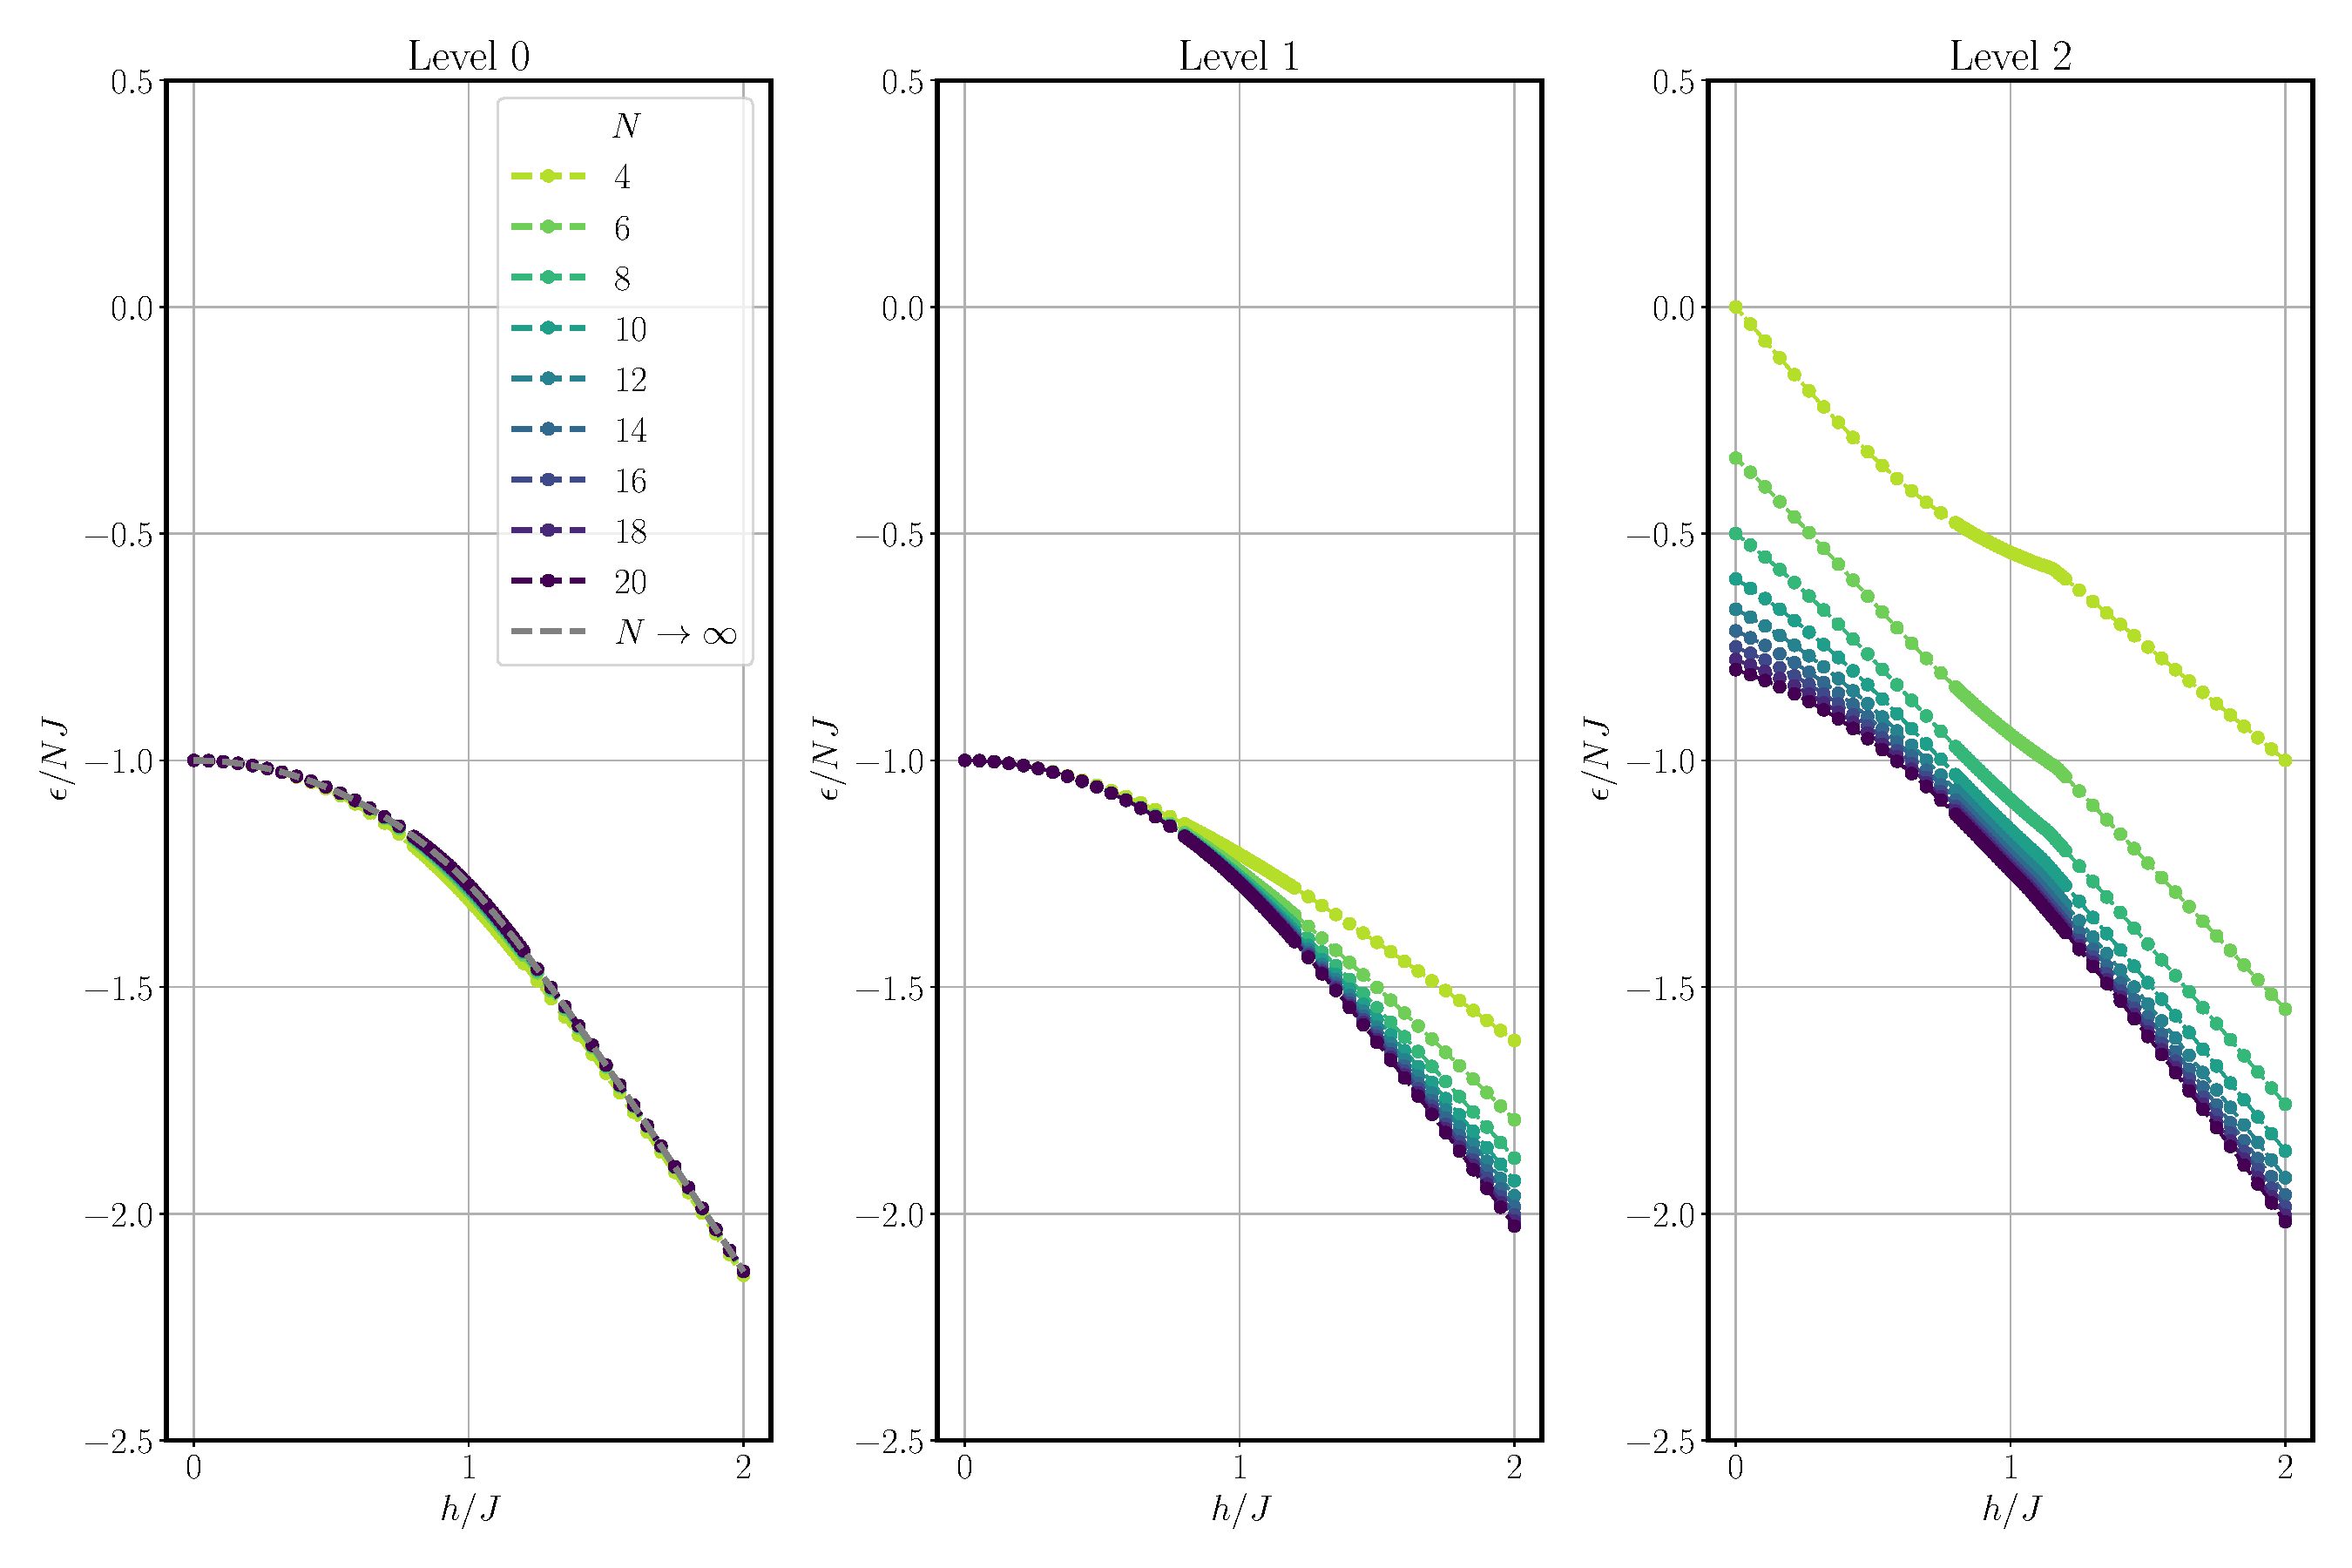
\includegraphics[width=1\textwidth]{figures/ising/energy__h__N.pdf}
  \caption{Energy per site as a function of the transverse field for various system sizes and energy levels, with the thermodynamic limit for the ground state energy shown \cite{Lieb1961}.}
  \label{fig:ising_energy_h_N}
\end{figure}


\subsection{Transverse Field Ising Model Order Parameter}
We now observe the trends in the order parameter in \cref{eq:ising_order} per site as a function of the transverse field. $64$ transverse fields, with denser field sampling around the hypothesized critical point of $\tilde{h}/J = 1$, and various system sizes $\leq 4 \leq N \leq 20$ are studied. Shown in \cref{fig:ising_order_h_N} are the order parameter for the first $3$ energy levels as per the sorted eigenvalues. 

We observe that the ground state at Level 0 order parameter obeys the exact limit of approaching $1$ as $h/J \to 0$, however there are significant finite size effects for the other limit of $h/J \to \infty$ as the order parameter appears to be approaching $0$, but very slowly. The convergence does accelerate for larger $N$, and for $N>16$ appears to somewhat converge to a similar curve that approaches $0$ slightly faster.

We also observe that the first excited state at Level 1 order parameter behaves similarly to the ground state, which makes sense if there is only infinitesimal splitting from the ground state for small $h/J$, however for $h/J > \tilde{h}/J$ there is also the expected trend of converging to a non-zero value. Similar to the ground state, there are significant finite-size effects, particularly for $N<10$, where energy level is almost constant with respect to $h/J$, and only for $N>16$ does some trend of convergence appear to occur.

For the second excited state at Level 2 order parameter has very interesting behaviour around the critical point of $\tilde{h}/J = 1$ and appears to diverge to a finite value. This appears to be similar divergences to other quantities such as the specific heat, which are generally measured with respect to the ground state at criticality, and perhaps there is a relation between the two divergences. Away from this critical region, the order parameter is roughly constant, and only shifted somewhat by finite size. These trends appear to be fairly independent of the system size.
\begin{figure}[H]
  \centering
  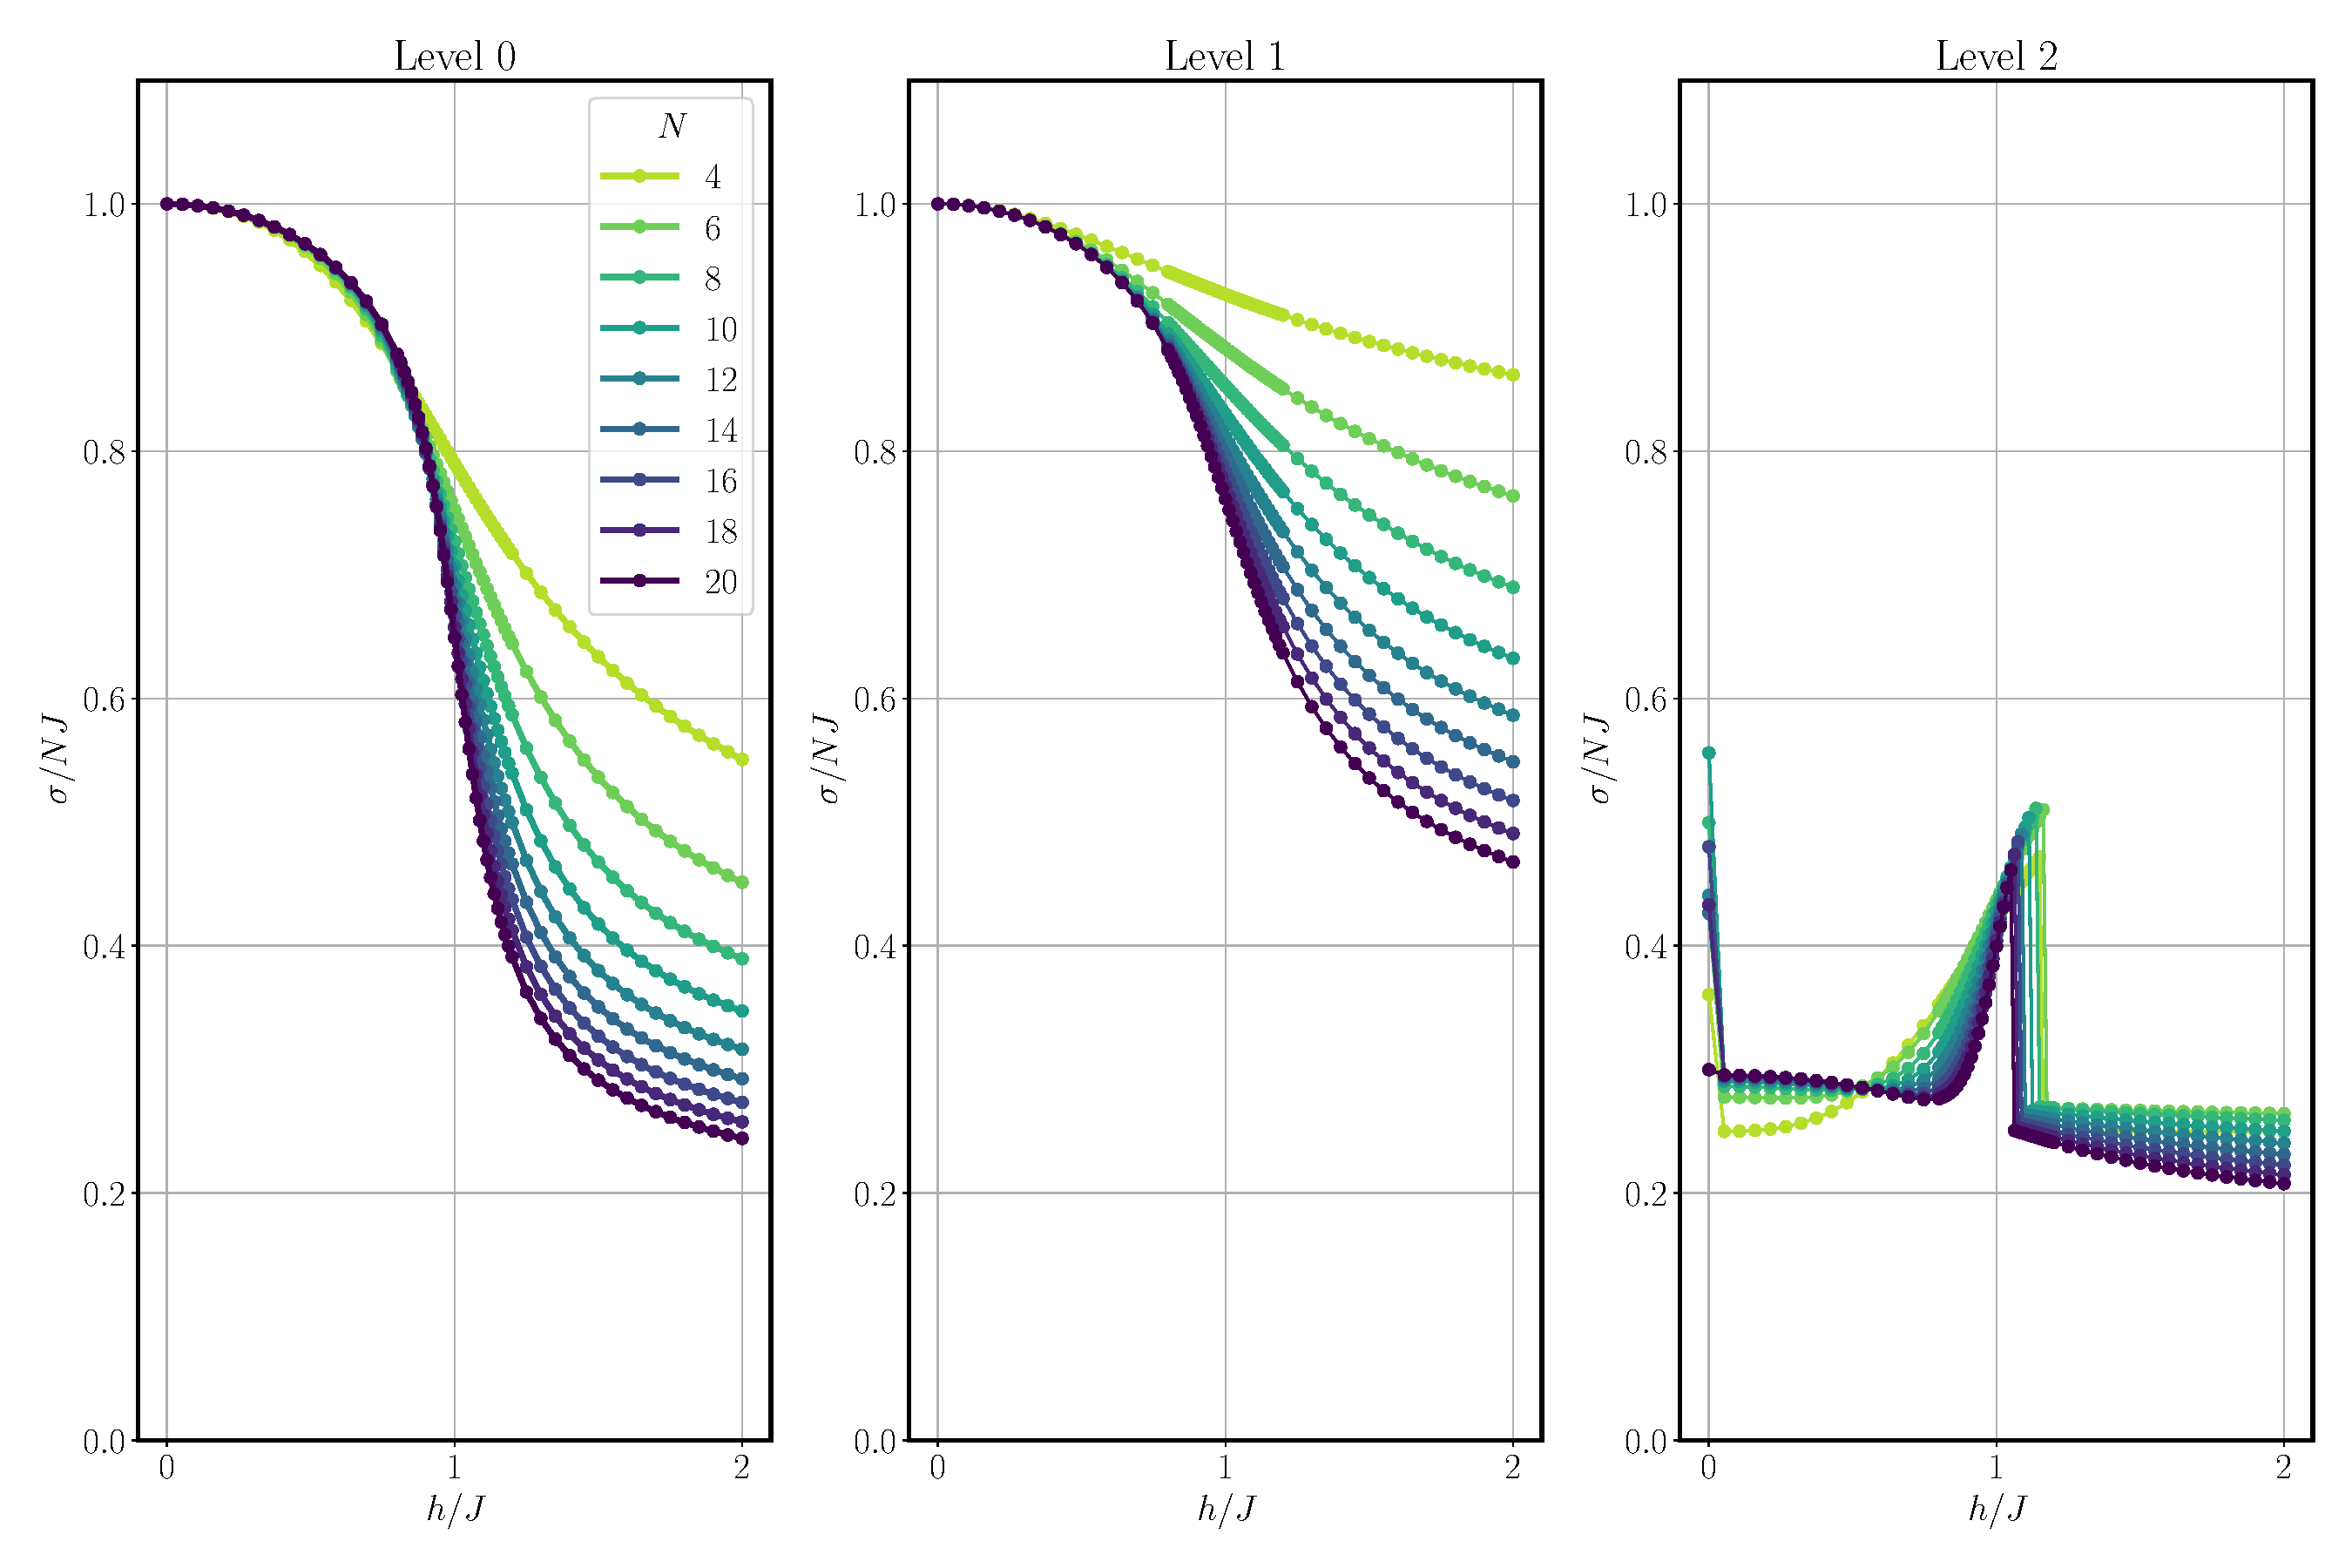
\includegraphics[width=1\textwidth]{figures/ising/order__h__N.pdf}
  \caption{Order parameter per site as a function of the transverse field for various system sizes and energy levels.}
  \label{fig:ising_order_h_N}
\end{figure}

\subsection{Transverse Field Ising Evidence of Phase Transition}
From the above analysis, there are several indications of different behaviour around a critical point of $\tilde{h}/J \approx 1$. First the order parameter changes curvature and approaches $0$ for $h/J > \tilde{h}/J$, and approaches a non-zero value for small $h/J$, indicating the predicted symmetry breaking towards one aligned phase of the spins. Further, the infinitesimal splitting between the ground state and first excited state for $h < \tilde{h}{J}$, relates to the predicted gap in the energy spectrum that is shown in \cref{eq:ising_gap} to be proportional to $\abs{h/J - \tilde{h}/J}$. The excitations with energy proportional to $h/J$ also fit with the previous analysis of the energy spectrum consisting of excitations of occupations of flipped spin states from the ground state.

\subsection{Transverse Field Ising Model Finite Size Scaling of Gap}
The gap between the TFIM ground state and first excited state around the hypothesized $\tilde{h}/J = 1$ critical point are now formally investigated. We assume a form of the scaling of the gap with finite size of
\begin{align}
  \Aboxed{\tilde{\Delta} \sim \tilde{\gamma}N^{-\tilde{z}} + \tilde{\delta}}~, \label{eq:ising_gap_model}
\end{align}
where the finite size critical exponent $\tilde{z}$, proportionality $\tilde{\gamma}$, and gap offset in the thermodynamic limit of $\tilde{\delta}$ are fitting parameters to be found. As per \cref{fig:ising_gap_N_h}, $16$ values of $0.9 \leq h/J \leq 1.1$, are used to determine the relation between the gap $\Delta$ as a function of $N$. 

For each transverse field the scaling parameters in \cref{eq:ising_gap_model} are fit. Given our knowledge that the gap should approach $\tilde{\Delta} \to 0$ in the thermodynamic limit at criticality, the transverse field that has the smallest absolute gap offset in the thermodynamic limit $\tilde{\delta} \approx 0$ is chosen as the predicted critical point given this data. This procedure reveals that the critical point is predicted to be
\begin{align}
  \Aboxed{\tilde{h}/J = 1}~, \label{eq:ising_criticalpt} \\
  \intertext{with finite size critical scaling parameters of}
  \Aboxed{\tilde{z} = 1.024}~, \\
  \Aboxed{\tilde{\gamma} = 1.633}~, \\
  \Aboxed{\tilde{\delta} = 0.003}~. 
\end{align}

\begin{figure}[H]
  \centering
  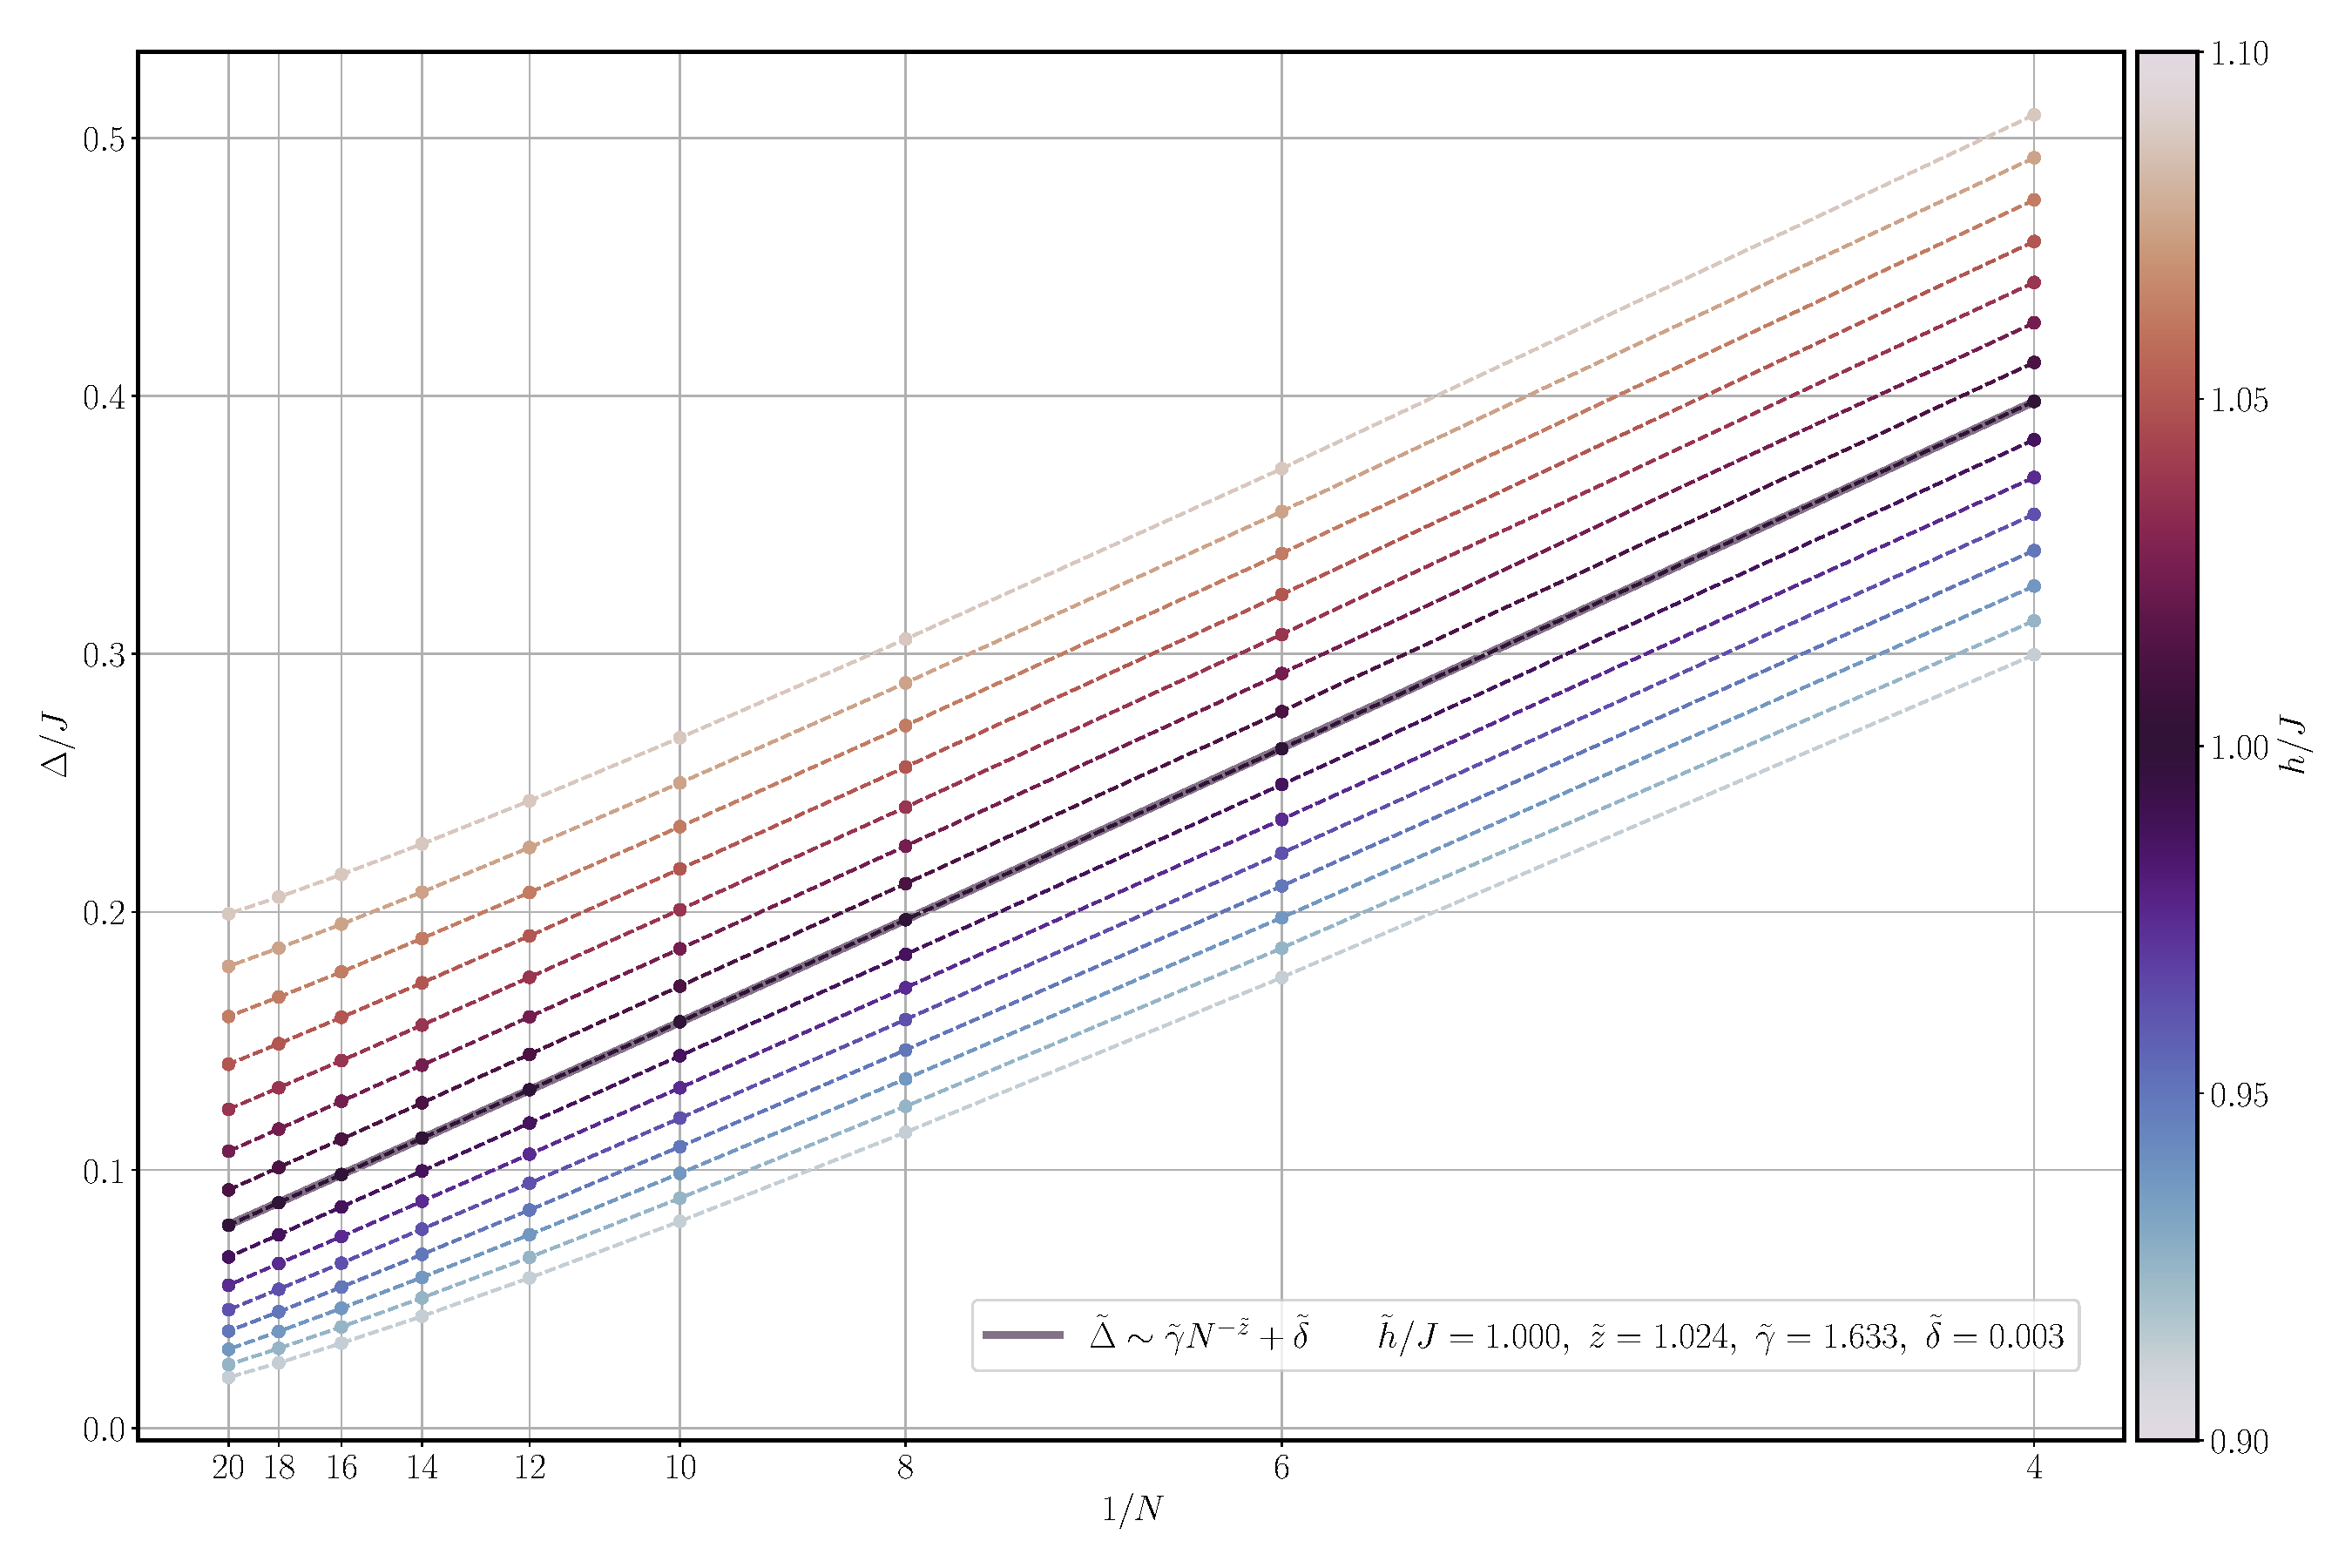
\includegraphics[width=1\textwidth]{figures/ising/gap__N__h.pdf}
  \caption{Gap between the ground state and first excited state as a function of the system size, for various transverse fields. The transverse field with the minimum gap offset in the thermodynamic limit and its scaling parameters is shown as the predicted critical point.}
  \label{fig:ising_gap_N_h}
\end{figure}
  
The fit coefficients of $\tilde{z}$ and $\tilde{\gamma}$ for the various transverse fields in \cref{fig:ising_gap_N_h} are found to be
\begin{figure}[H]
  \centering
  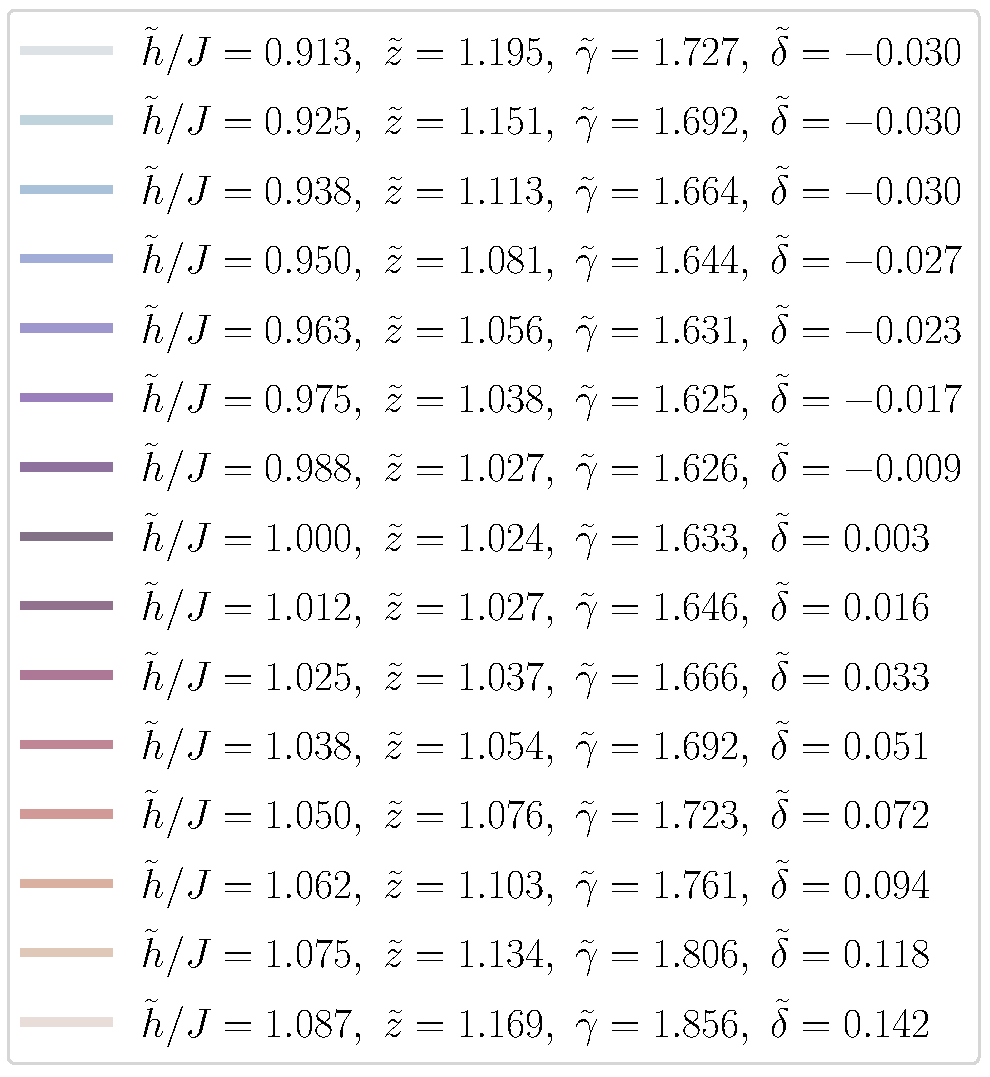
\includegraphics[width=0.4\textwidth]{figures/ising/gap__N__h_legend.pdf}
  \label{fig:ising_gap_N_h_legend}
\end{figure}
and are found to be quite constant around $\tilde{z} \approx 1$, and $\tilde{\gamma} \approx 1.6$, indicating the ansatz was appropriate. The finite size effects are also shown to predominately affect the magnitude of gap at the critical point, and not the position of the gap. Furthermore, the gap offsets are approximately symmetric about the minimum value, being positive for $h/J< \tilde{h}/J$, and positive for $h/J > \tilde{h}/J$. 

Therefore it is claimed that there is a critical point at $\tilde{h}/J = 1$, and that gap has a finite size scaling of approaching zero at this critical point as
\begin{align}
  \Aboxed{\tilde{\Delta} \sim N^{-1}}~, \label{eq:ising_criticalscaling}
\end{align}
Therefore this finite scaling analysis agrees with the theoretical predictions of the critical behaviour of the TFIM, and is a sound approach. An improved approach would be conducting a full finite-size scaling with an ansatz about a universal scaling function, and using a data-collapse method to prove the universality of the critical exponents and obtain improved estimates.

\newpage
\section{Anisotropic Heisenberg Models}
We now investigate the ground state properties of the Anisotropic Heisenberg model (XXZ). Identical to the TFIM model, we exactly diagonalize the XXZ Hamiltonian, and compute observables such as the ground state energy from the eigenvalues and eigenvectors. 

\subsection{Anisotropic Heisenberg Model Subspaces}
As discussed in the introduction, the XXZ model, for limits of the couplings within the paramagnetic phase, has a non-degenerate unique ground state with $S^{z} = 0$, which can be shown to exist from the $U_z(1)$ symmetry present in the model, as well as the positivity of the ground state coefficients. justified to study the $S^{z} = 0$ subspace, and make conclusions about the ground state properties based on the eigenstates within this subspace. We are also able to study larger system sizes since the data structure sizes now only scale with the subspace dimension of $N!/(N/2)!^2 < 2^N$.

\subsection{Anisotropic Heisenberg Model Ground State Energy}
We will focus on the finite-size scaling of the ground state energy $\Omega$ for the XY and AH models as function of system size $4 \leq N \leq 24$, based on the known ground state energies in the thermodynamic limit of $\Omega_{XY}/{NJ} = -1/\pi$ and $\Omega_{AH}/{NJ} = 1/4 - \log2$ in \cref{eq:xy_groundenergy} and \cref{eq:ah_groundenergy}. Given this relation, we will assume a power-law scaling relation for finite size $N$ of
\begin{align}
  \frac{\Omega_{\textrm{XY,AH}}}{NJ} =&~ \bar{\alpha} N^{-\bar{\lambda}} + \bar{\Omega}, \label{eq:xyah_energyscaling}
\end{align}
where $\bar{\Omega}$ should approach the thermodynamic limits in \cref{eq:xy_groundenergy} and \cref{eq:ah_groundenergy}, and $\bar{\lambda}$ and $\bar{\alpha}$ represent the power-law scaling to approach these limits.

Shown in \cref{fig:xy_energy_N} and \cref{fig:ah_energy_N} are the ground state energies as a function of system size $N$ for the XY and AH models respectively, with the fit scaling relations of \cref{eq:xyah_energyscaling} shown compared to the thermodynamic limits.
\begin{figure}[H]
  \centering
  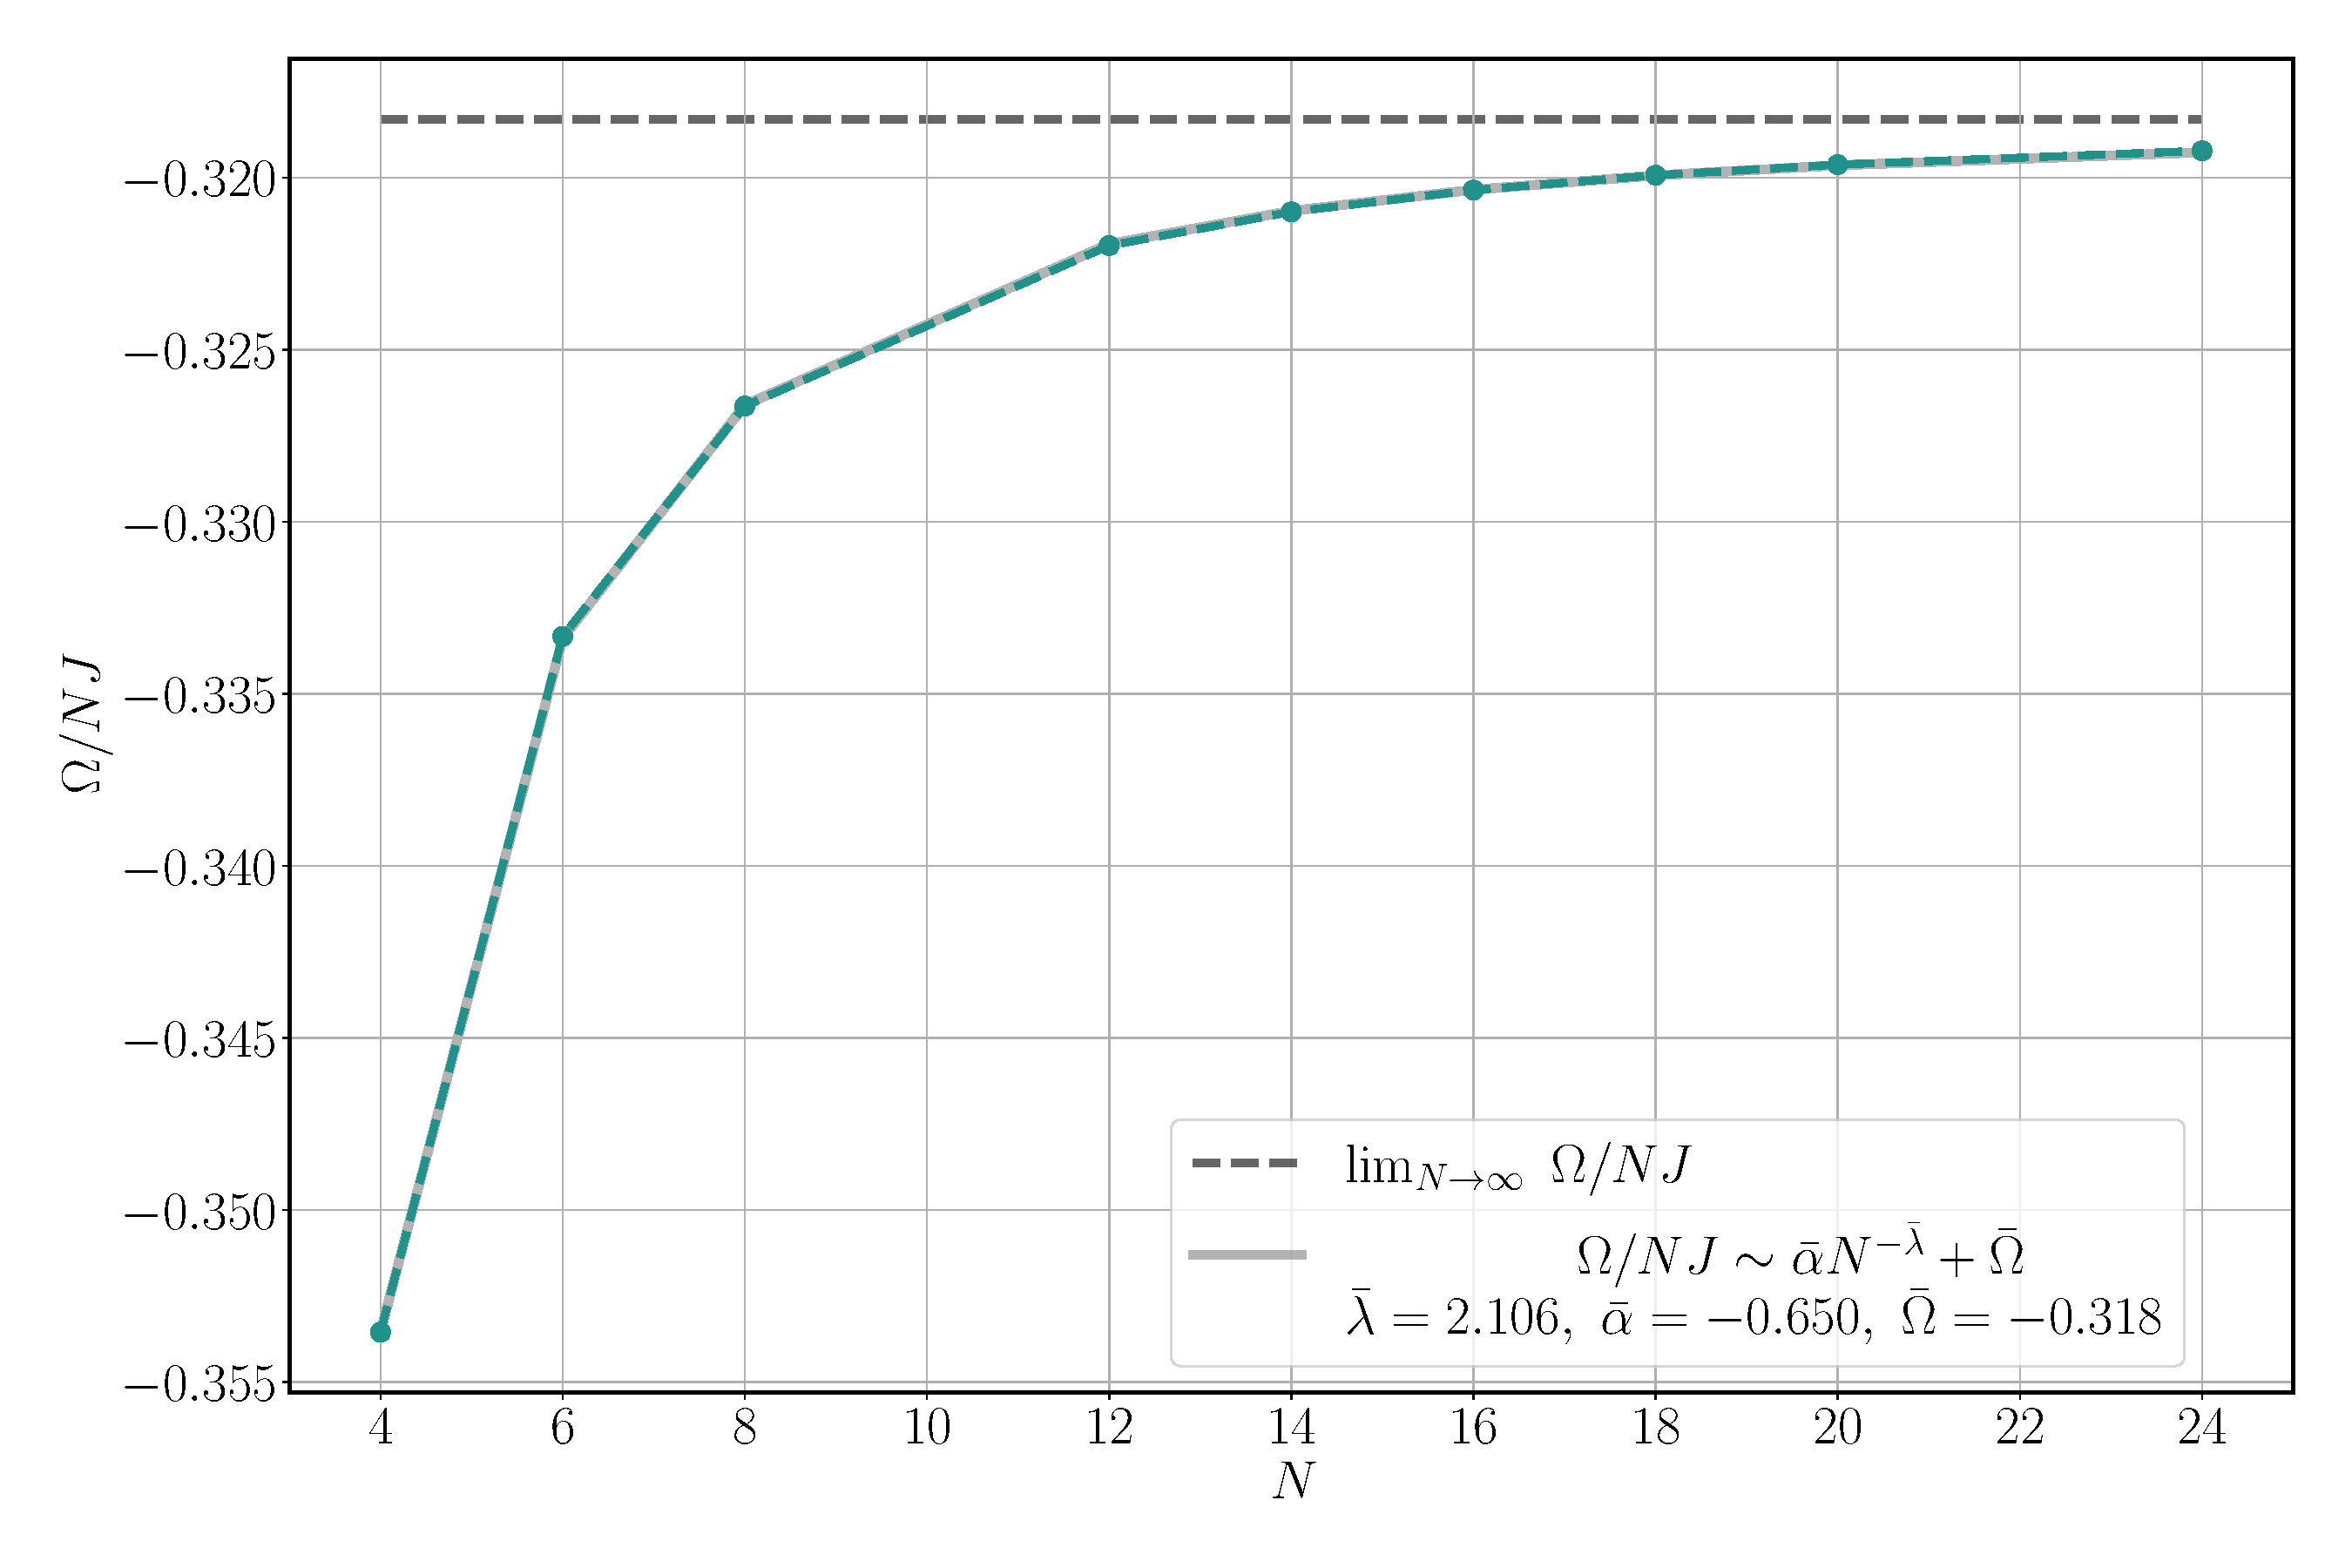
\includegraphics[width=0.8\textwidth]{figures/xy/energy__N__U.pdf}
  \caption{Ground state energy per site as a function of the system size for the XY model, with the thermodynamic limit for the ground state energy shown \cite{Lieb1961}.}
  \label{fig:xy_energy_N}
\end{figure}
\begin{figure}[H]
  \centering
  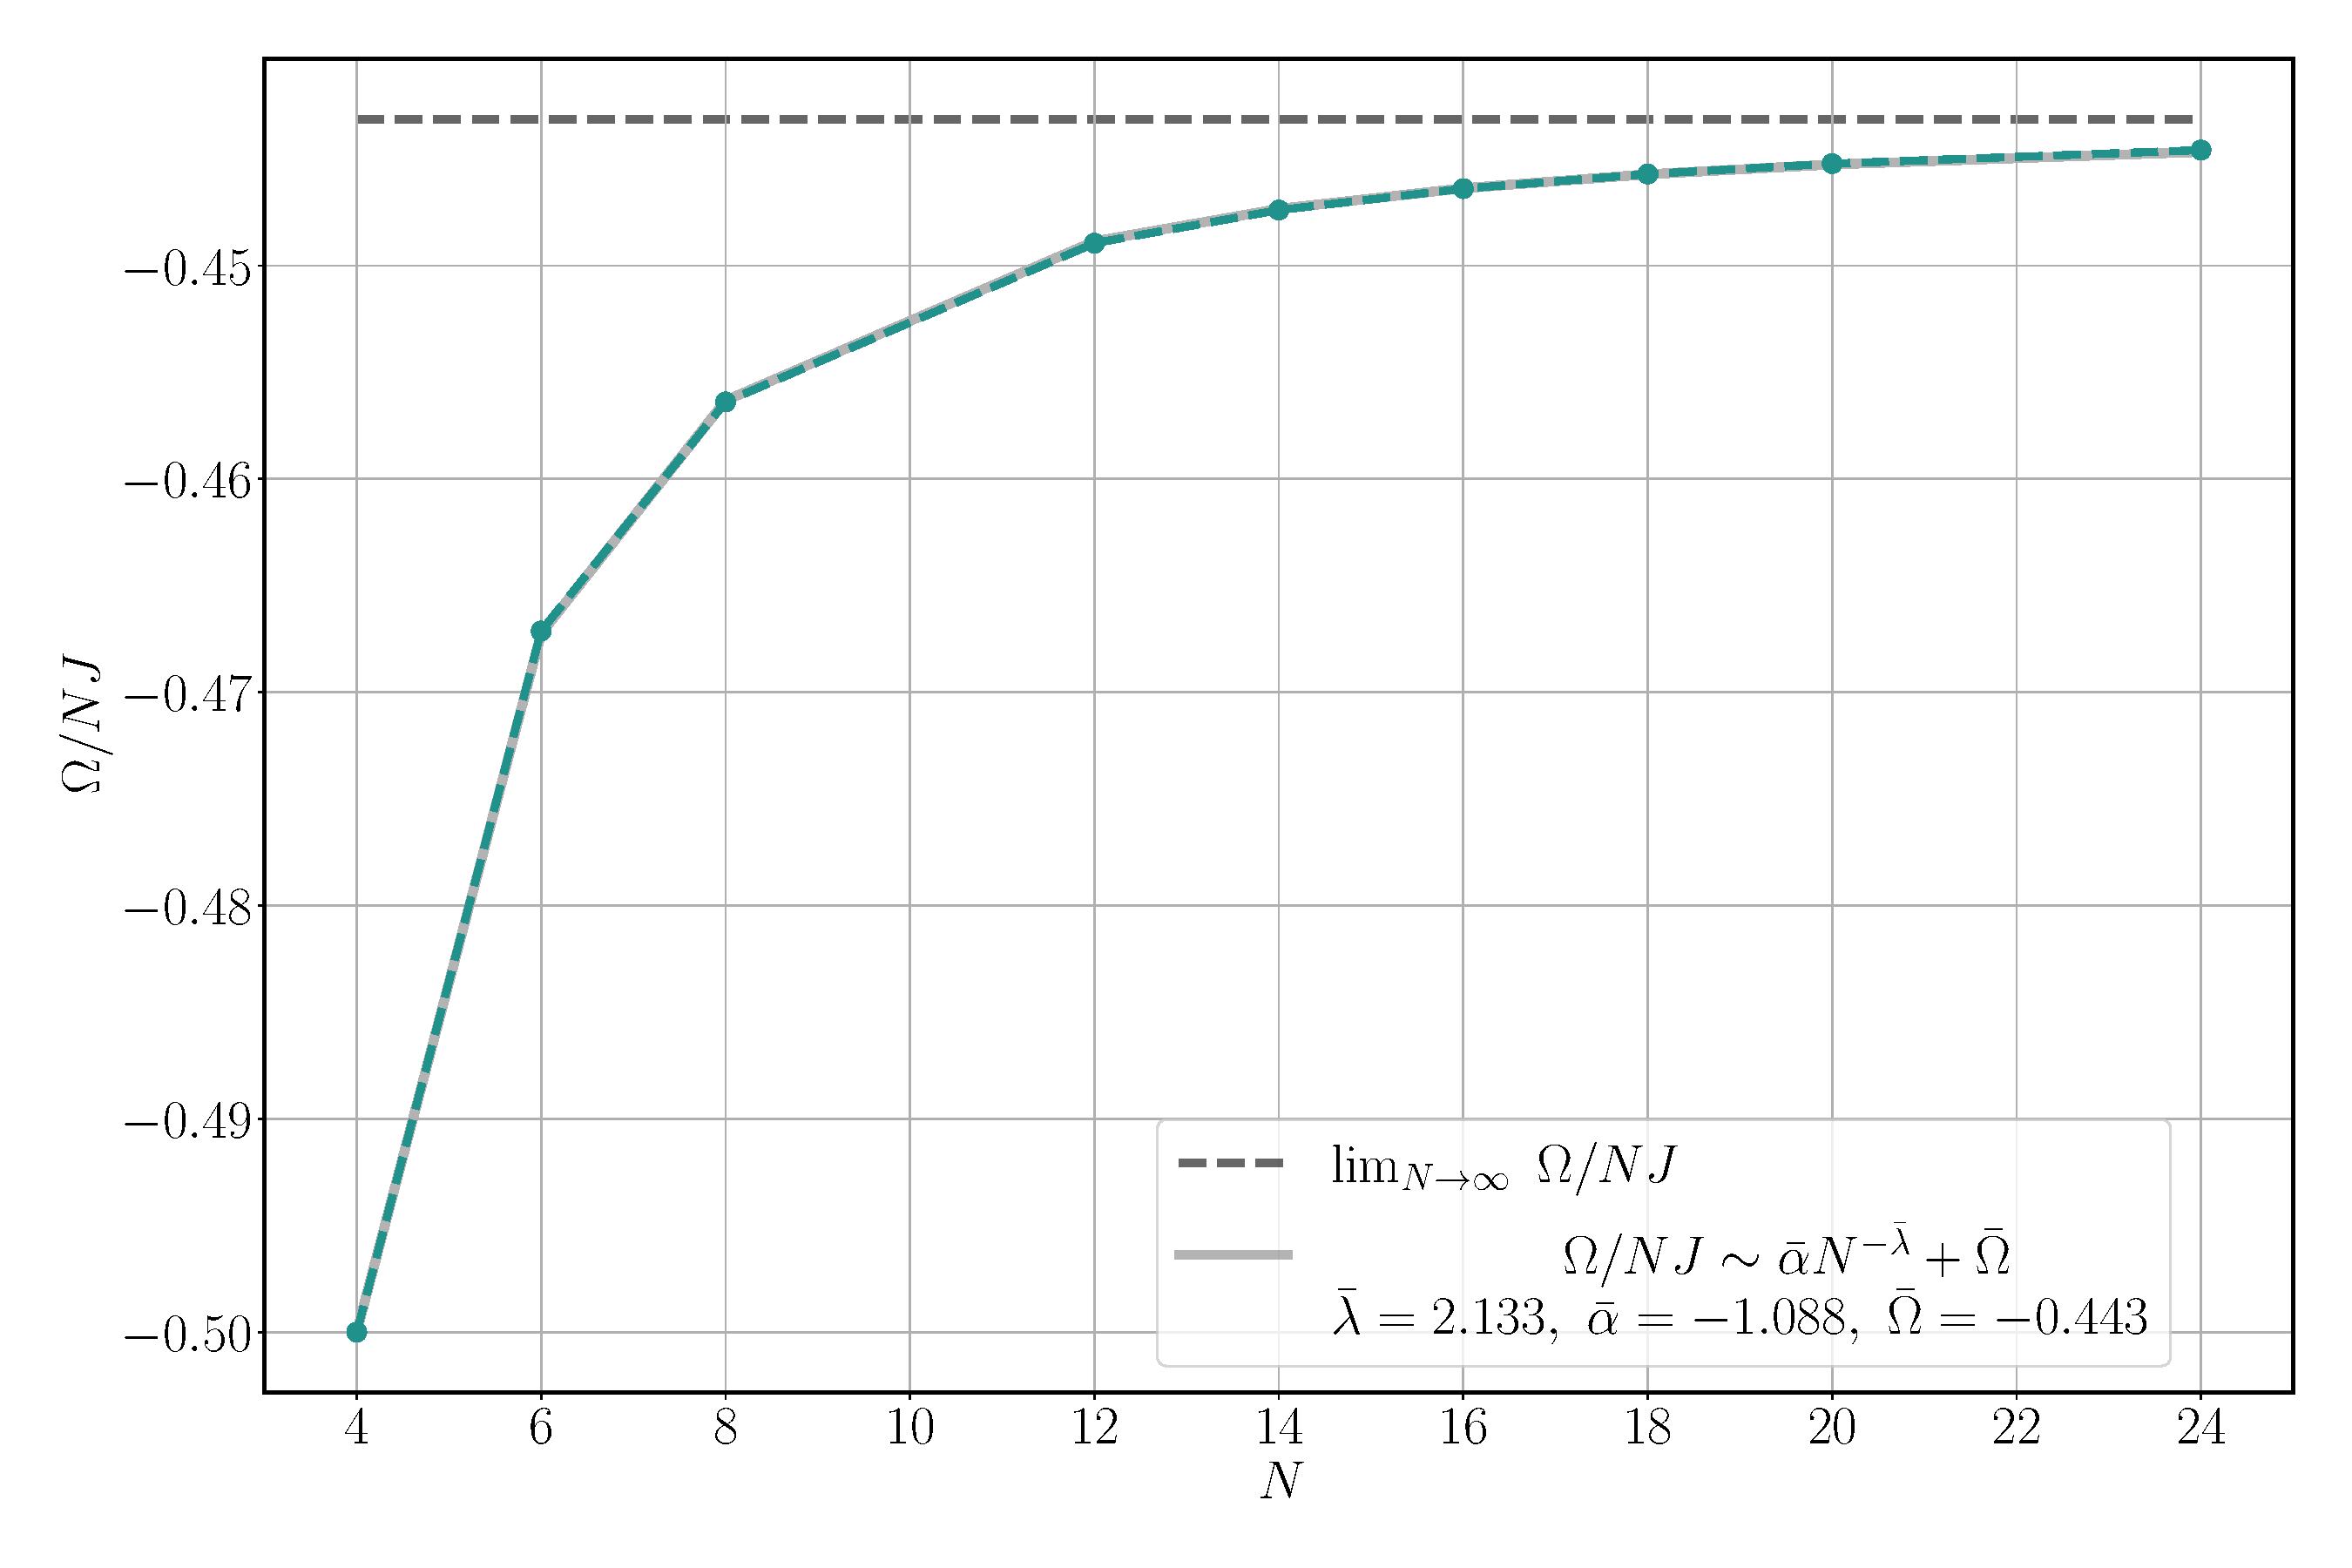
\includegraphics[width=0.8\textwidth]{figures/ah/energy__N__U.pdf}
  \caption{Ground state energy per site as a function of the system size for the AH model, with the thermodynamic limit for the ground state energy shown \cite{Lieb1961}.}
  \label{fig:ah_energy_N}
\end{figure}

For $N>16$, both the finite size XY and AH models approaches their thermodynamic limit ground state energies quickly. It can be seen that the power-law ansatz is appropriate, with a power law where the finite size ground state energy decays \emph{quadratically} to its thermodynamic limit
\begin{align}
  \Aboxed{\frac{\Omega_{XY,AH}}{NJ} \sim N^{-2}}~, \label{eq:xyah_energyscaling_fit} \\
  \intertext{with relative error of the fitted thermodynmic limits of approximately}
  \abs{\frac{\bar{\Omega}_{XY} - \Omega_{\textrm{XY}}/{NJ}}{\Omega_{\textrm{XY}}/{NJ}}} =&~ 0.02, \\
  \abs{\frac{\bar{\Omega}_{AH} - \Omega_{\textrm{AH}}/{NJ}}{\Omega_{\textrm{AH}}/{NJ}}} =&~ 0.001.
\end{align}
Therefore this analysis shows the finite size ground state energies of models within the paramagnetic phase, approach the thermodynamic limit quadratically with system size. Similar to the critical scaling analysis of the TFIM model, an ansatz about a universal scaling function for these quantities would allow for a data-collapse approach to more rigorously confirm these types of scalings.

\newpage
\section{Entanglement Entropy and Central Charges}
We now bipartition our systems, and as per the reshaping and partial trace procedure outlined in \cref{eq:reduced_rho} and \cref{eq:svd}, calculate the entanglement entropy of the bipartition. Ultimately, we desire the scaling of the entanglement entropy as per \cref{eq:entropy_scaling} of $S = c \frac{1}{3}\log{\left(\frac{L}{\pi} \sin{(\pi \frac{L}{N})}\right)} + C$. 

\subsection{Transverse Field Ising Model Entanglement Scaling}
We first investigate the scaling of the entanglement entropy for the TFIM model. Shown in \cref{fig:ising_entanglement_partition} is the entanglement entropy scaling for $4 \leq N \leq 20$ and $h/J = 0,\tilde{h}/J,2$. We observe the critical entanglement behaviour fits almost perfectly with the scaling in \cref{eq:entropy_scaling}, and the central charge approaches the known value \cite{Cole2017} of $\boxed{c_{\textrm{TFIM}} = 1/2}$ as the system size increases, and particularly converges for $N>14$. The entanglement is also seen to be maximized at this critical transverse field.

At $h/J = 0 < \tilde{h}/J$, it can be seen that the entanglement is constant for all bipartition sizes $L$, and for this particular value of zero transverse field, identical to in the finite size analysis of the TFIM energy spectrum, the finite size allows for perturbative tunnelling between both states, and some linear combinations of the these two ground states spanning this degenerate subspace $\ket{\Omega} = \alpha \ket{\uparrow} + \beta \ket{\downarrow}$ are found by the eigen-solver for the two lowest energy eigenstates. The entanglement entropy at zero transverse field should be $S = 0$ if symmetry breaking occurs and there is a unique ground state with spins all oriented along one direction, however it is off by a constant factor of $S = -2(\alpha^2\log\alpha + \beta^2\log\beta)$, where $\alpha,\beta$ are real coefficients for any normalized state within this subspace.

For $h/J > \tilde{h}{J}$, it can be seen that the entanglement is constant for bipartitions of size $0 \ll L/N \ll 1$, and only when one of the bipartitions is relatively much larger does the entanglement decrease. This suggests a more volume-like law. Further, at higher $h/J$ as the spins become more aligned along the $x$ direction, they become less entangled and the magnitude of the entanglement also approaches zero.

\begin{figure}[H]
  \centering
  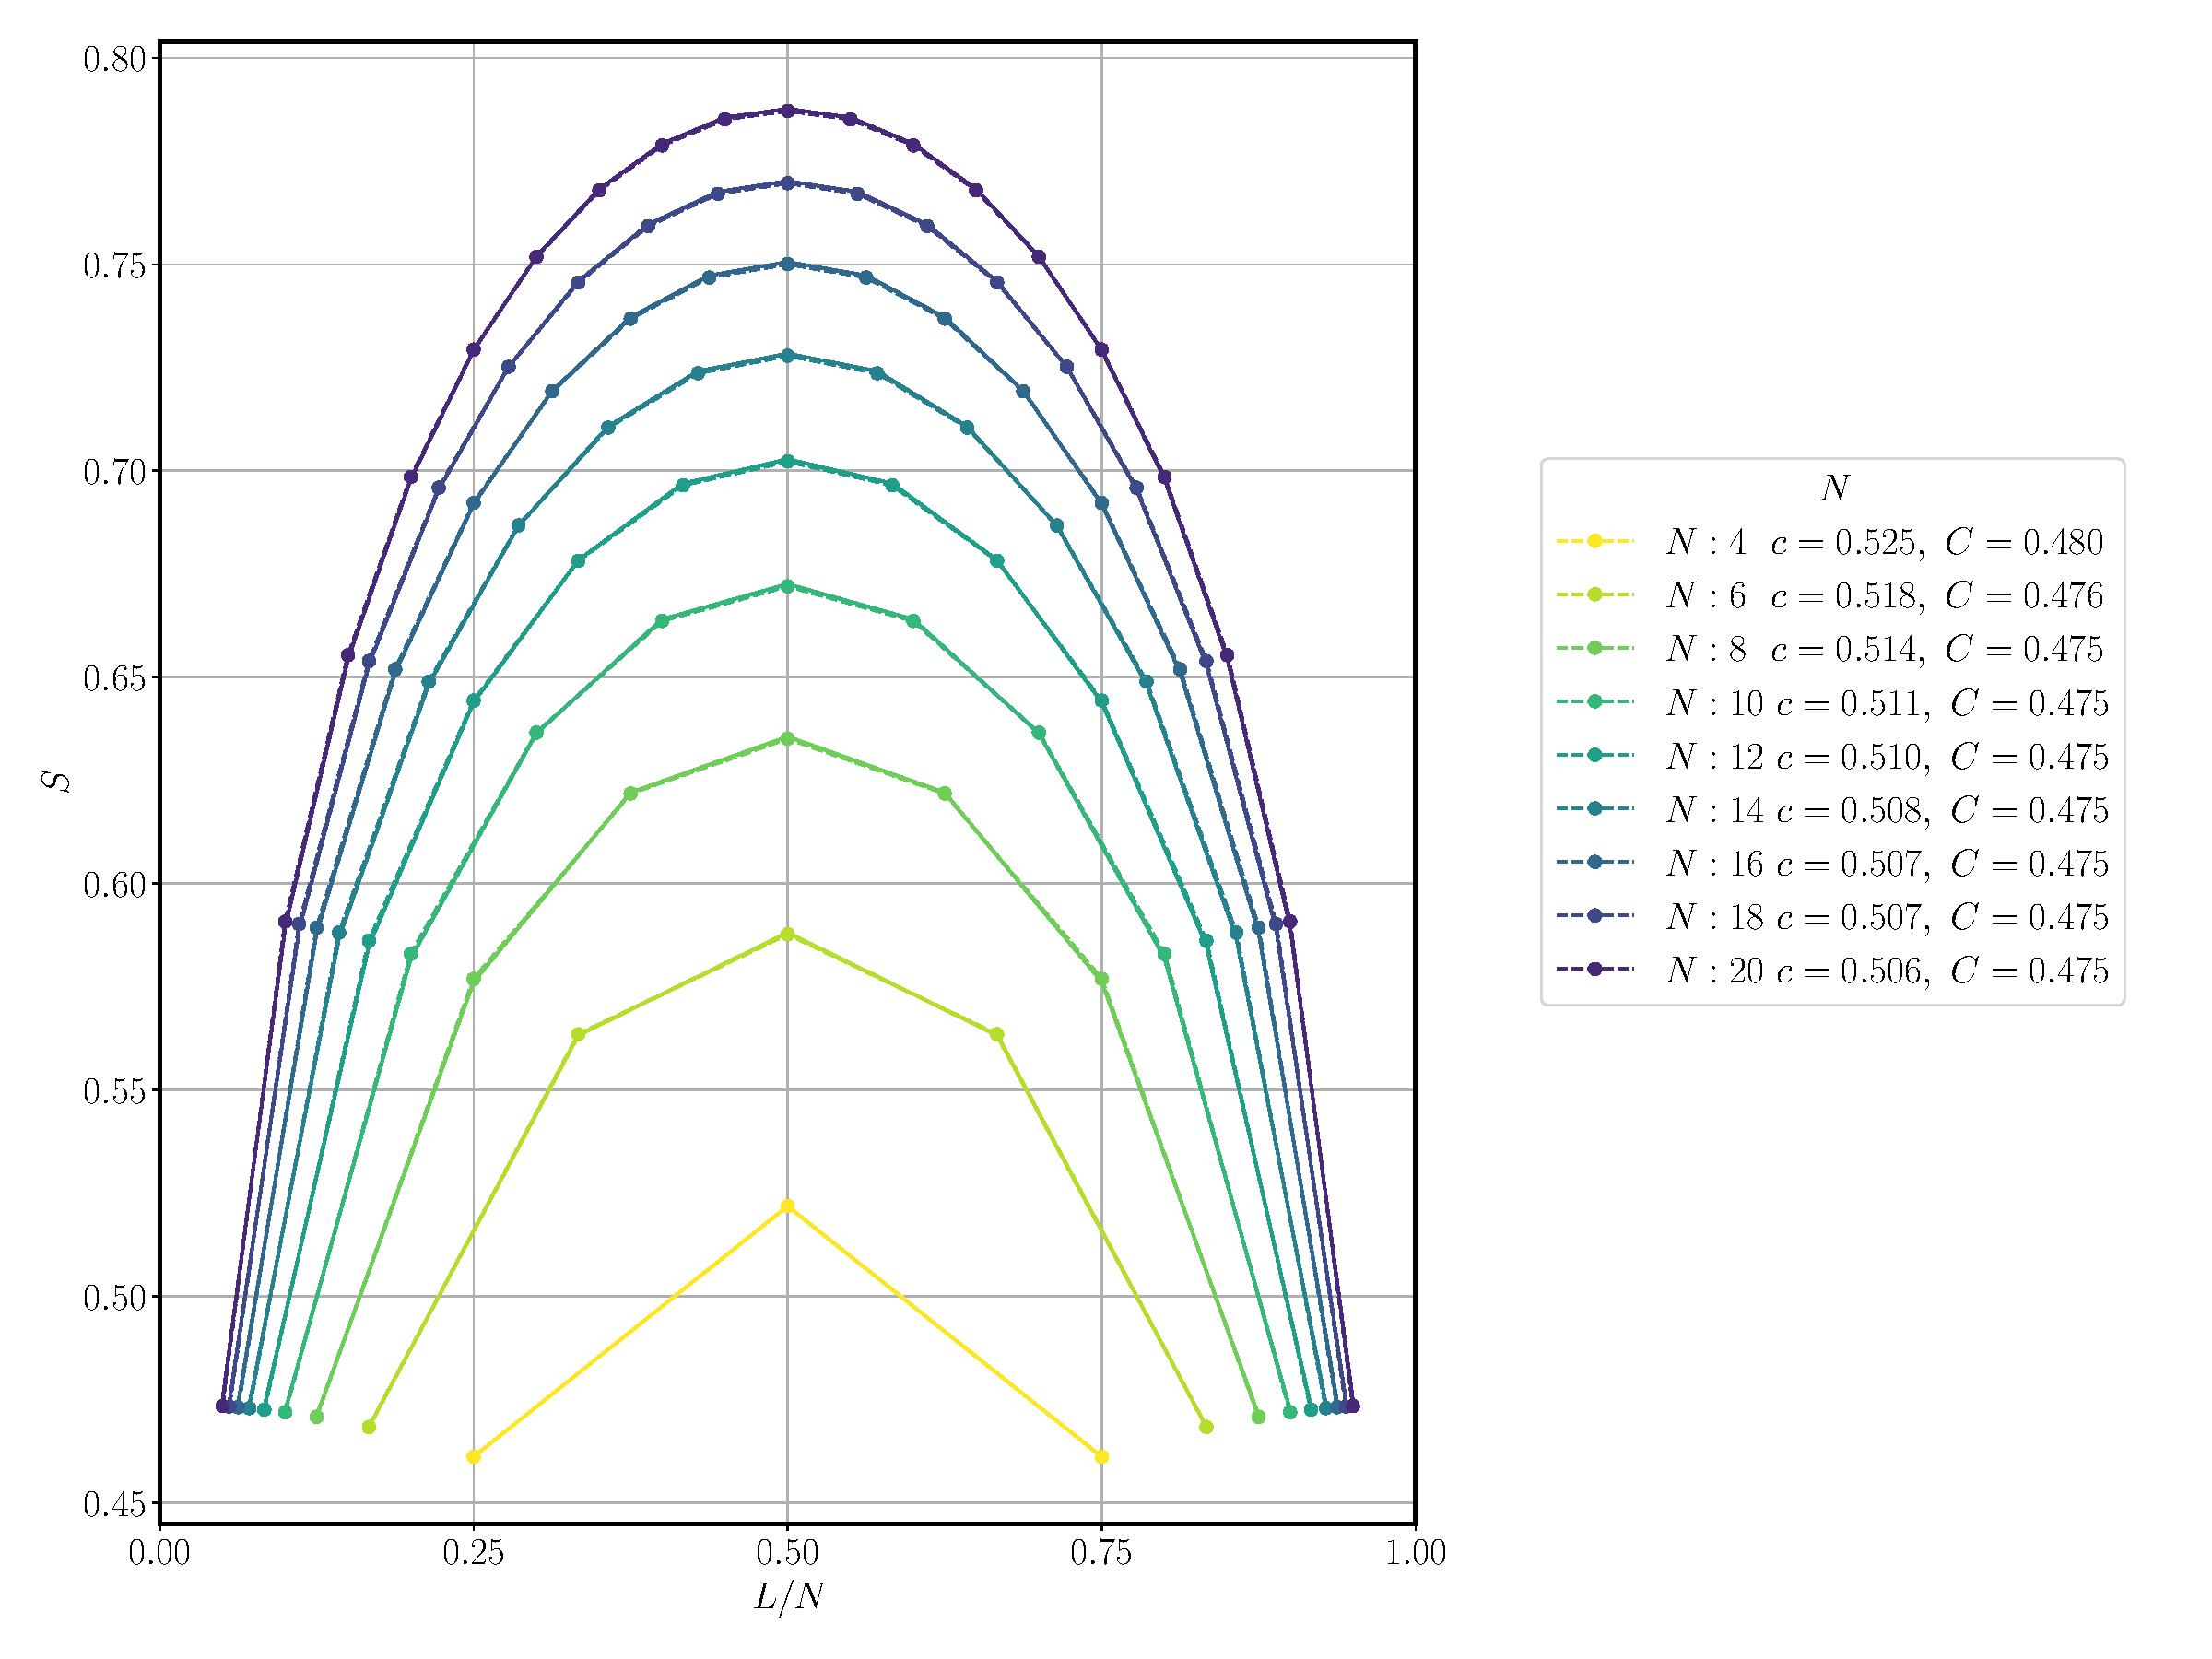
\includegraphics[width=1\textwidth]{figures/ising/entanglement__partition__N.pdf}
  \caption{Entanglement entropy for the TFIM model as a function of the partition size, for various system sizes and transverse fields. Shown are fitted curves of the entanglement scaling relation at criticality $\tilde{h}/J$, with fitted central charges and corrections.}
  \label{fig:ising_entanglement_partition}
\end{figure}


\subsection{XY Model Entanglement Scaling}
We now investigate the scaling of the entanglement entropy for the XY model. Shown in \cref{fig:xy_entanglement_partition} is the entanglement entropy scaling for $4 \leq N \leq 24$. We observe the entanglement behaviour fits almost perfectly with the scaling in \cref{eq:entropy_scaling}, and the central charge approaches the known value \cite{Cole2017} of $\boxed{c_{\textrm{XY}} = 1}$ as the system size increases, and particularly converges for $N>14$. This model is confirmed to be within the paramagnetic anisotropic Heisenberg model universality class, and is exhibiting some kind of critical behaviour if its entanglement is scaling as if it is conformal. It is also interesting to observe that the corrections $C$ appear to be independent of system size, indicating that if there are any corrections, they may only depend on dimensionless ratios $L/N$.
\begin{figure}[H]
  \centering
  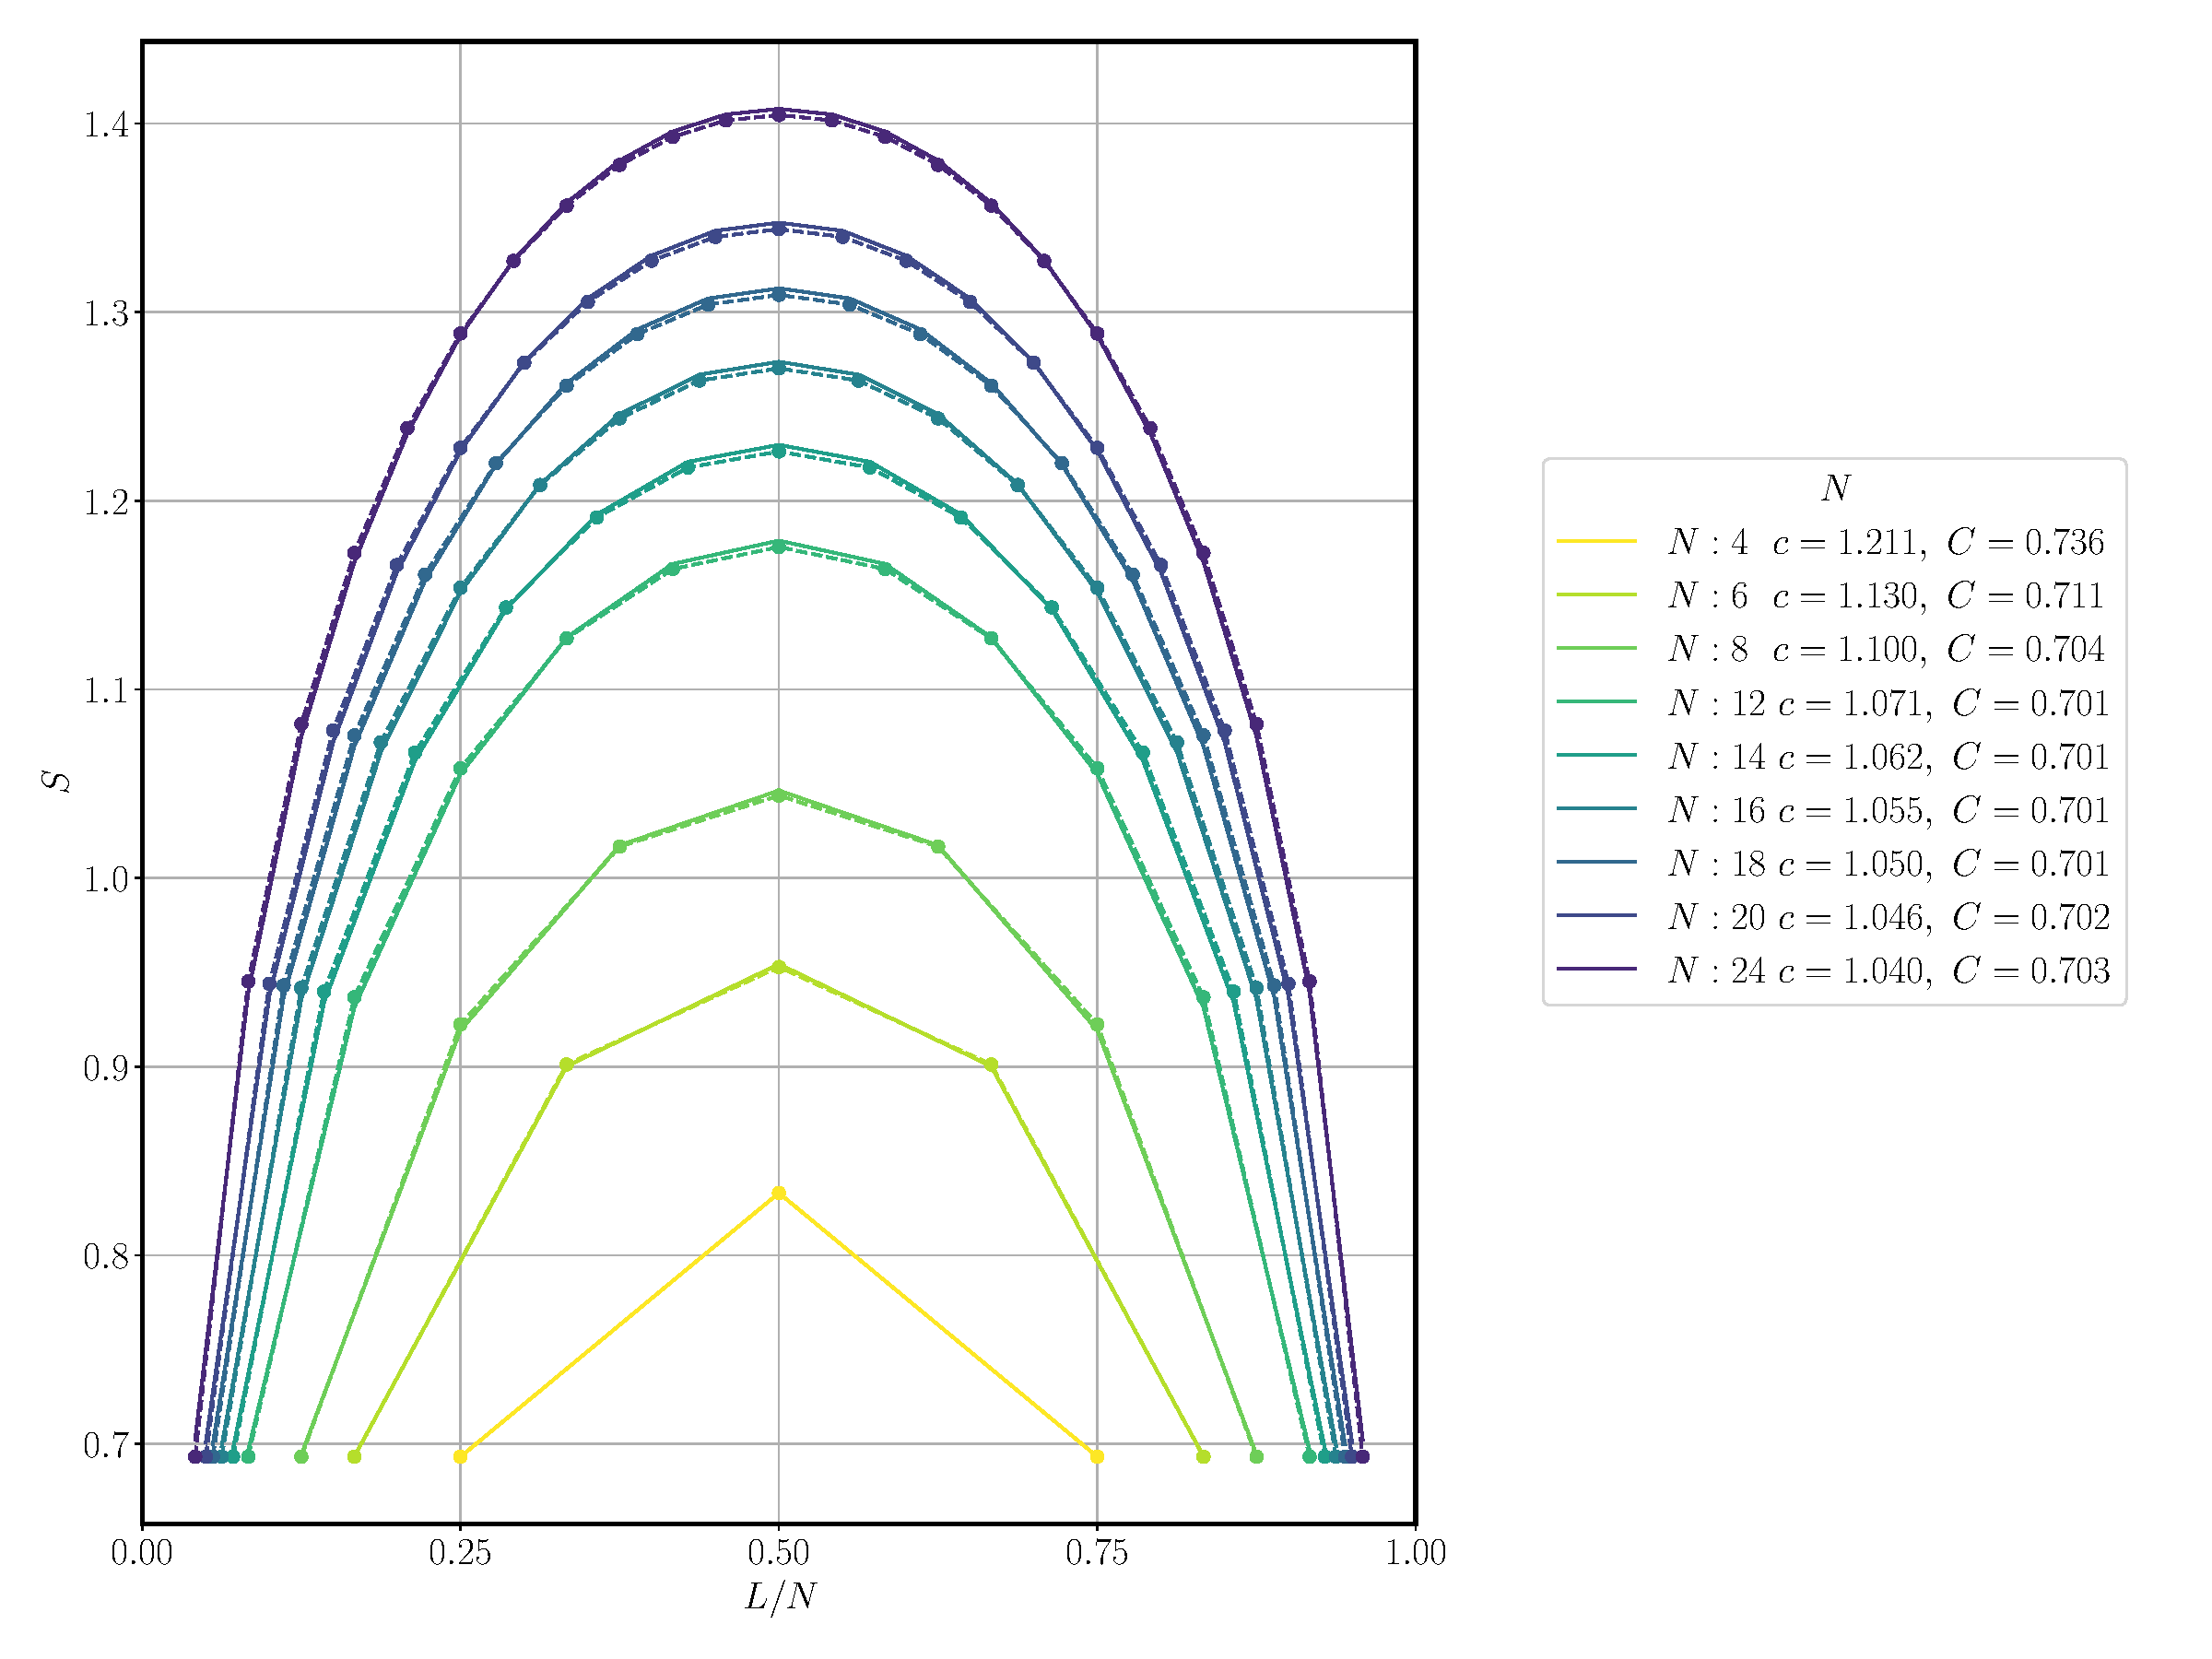
\includegraphics[width=1\textwidth]{figures/xy/entanglement__partition__N__U__J.pdf}
  \caption{Entanglement entropy for the XY model as a function of the partition size, for various system sizes. Shown are fitted curves of the entanglement scaling relation, with fitted central charges and corrections.}
  \label{fig:xy_entanglement_partition}
\end{figure}

\subsection{AH Model Entanglement Scaling}
We now investigate the scaling of the entanglement entropy for the AH model. Shown in \cref{fig:ah_entanglement_partition} is the entanglement entropy scaling for $4 \leq N \leq 24$. We observe the entanglement behaviour fits almost perfectly with the scaling in \cref{eq:entropy_scaling}, and the central charge approaches the known value \cite{Cole2017} of $\boxed{c_{\textrm{AH}} = 1}$ as the system size increases, and particularly converges for $N>14$. This model is confirmed to be within the paramagnetic anisotropic Heisenberg model universality class, and is exhibiting some kind of critical behaviour if its entanglement is scaling as if it is conformal. It is also interesting to observe that the corrections $C$ appear to be independent of system size, indicating that if there are any corrections, they may only depend on dimensionless ratios $L/N$.
\begin{figure}[H]
  \centering
  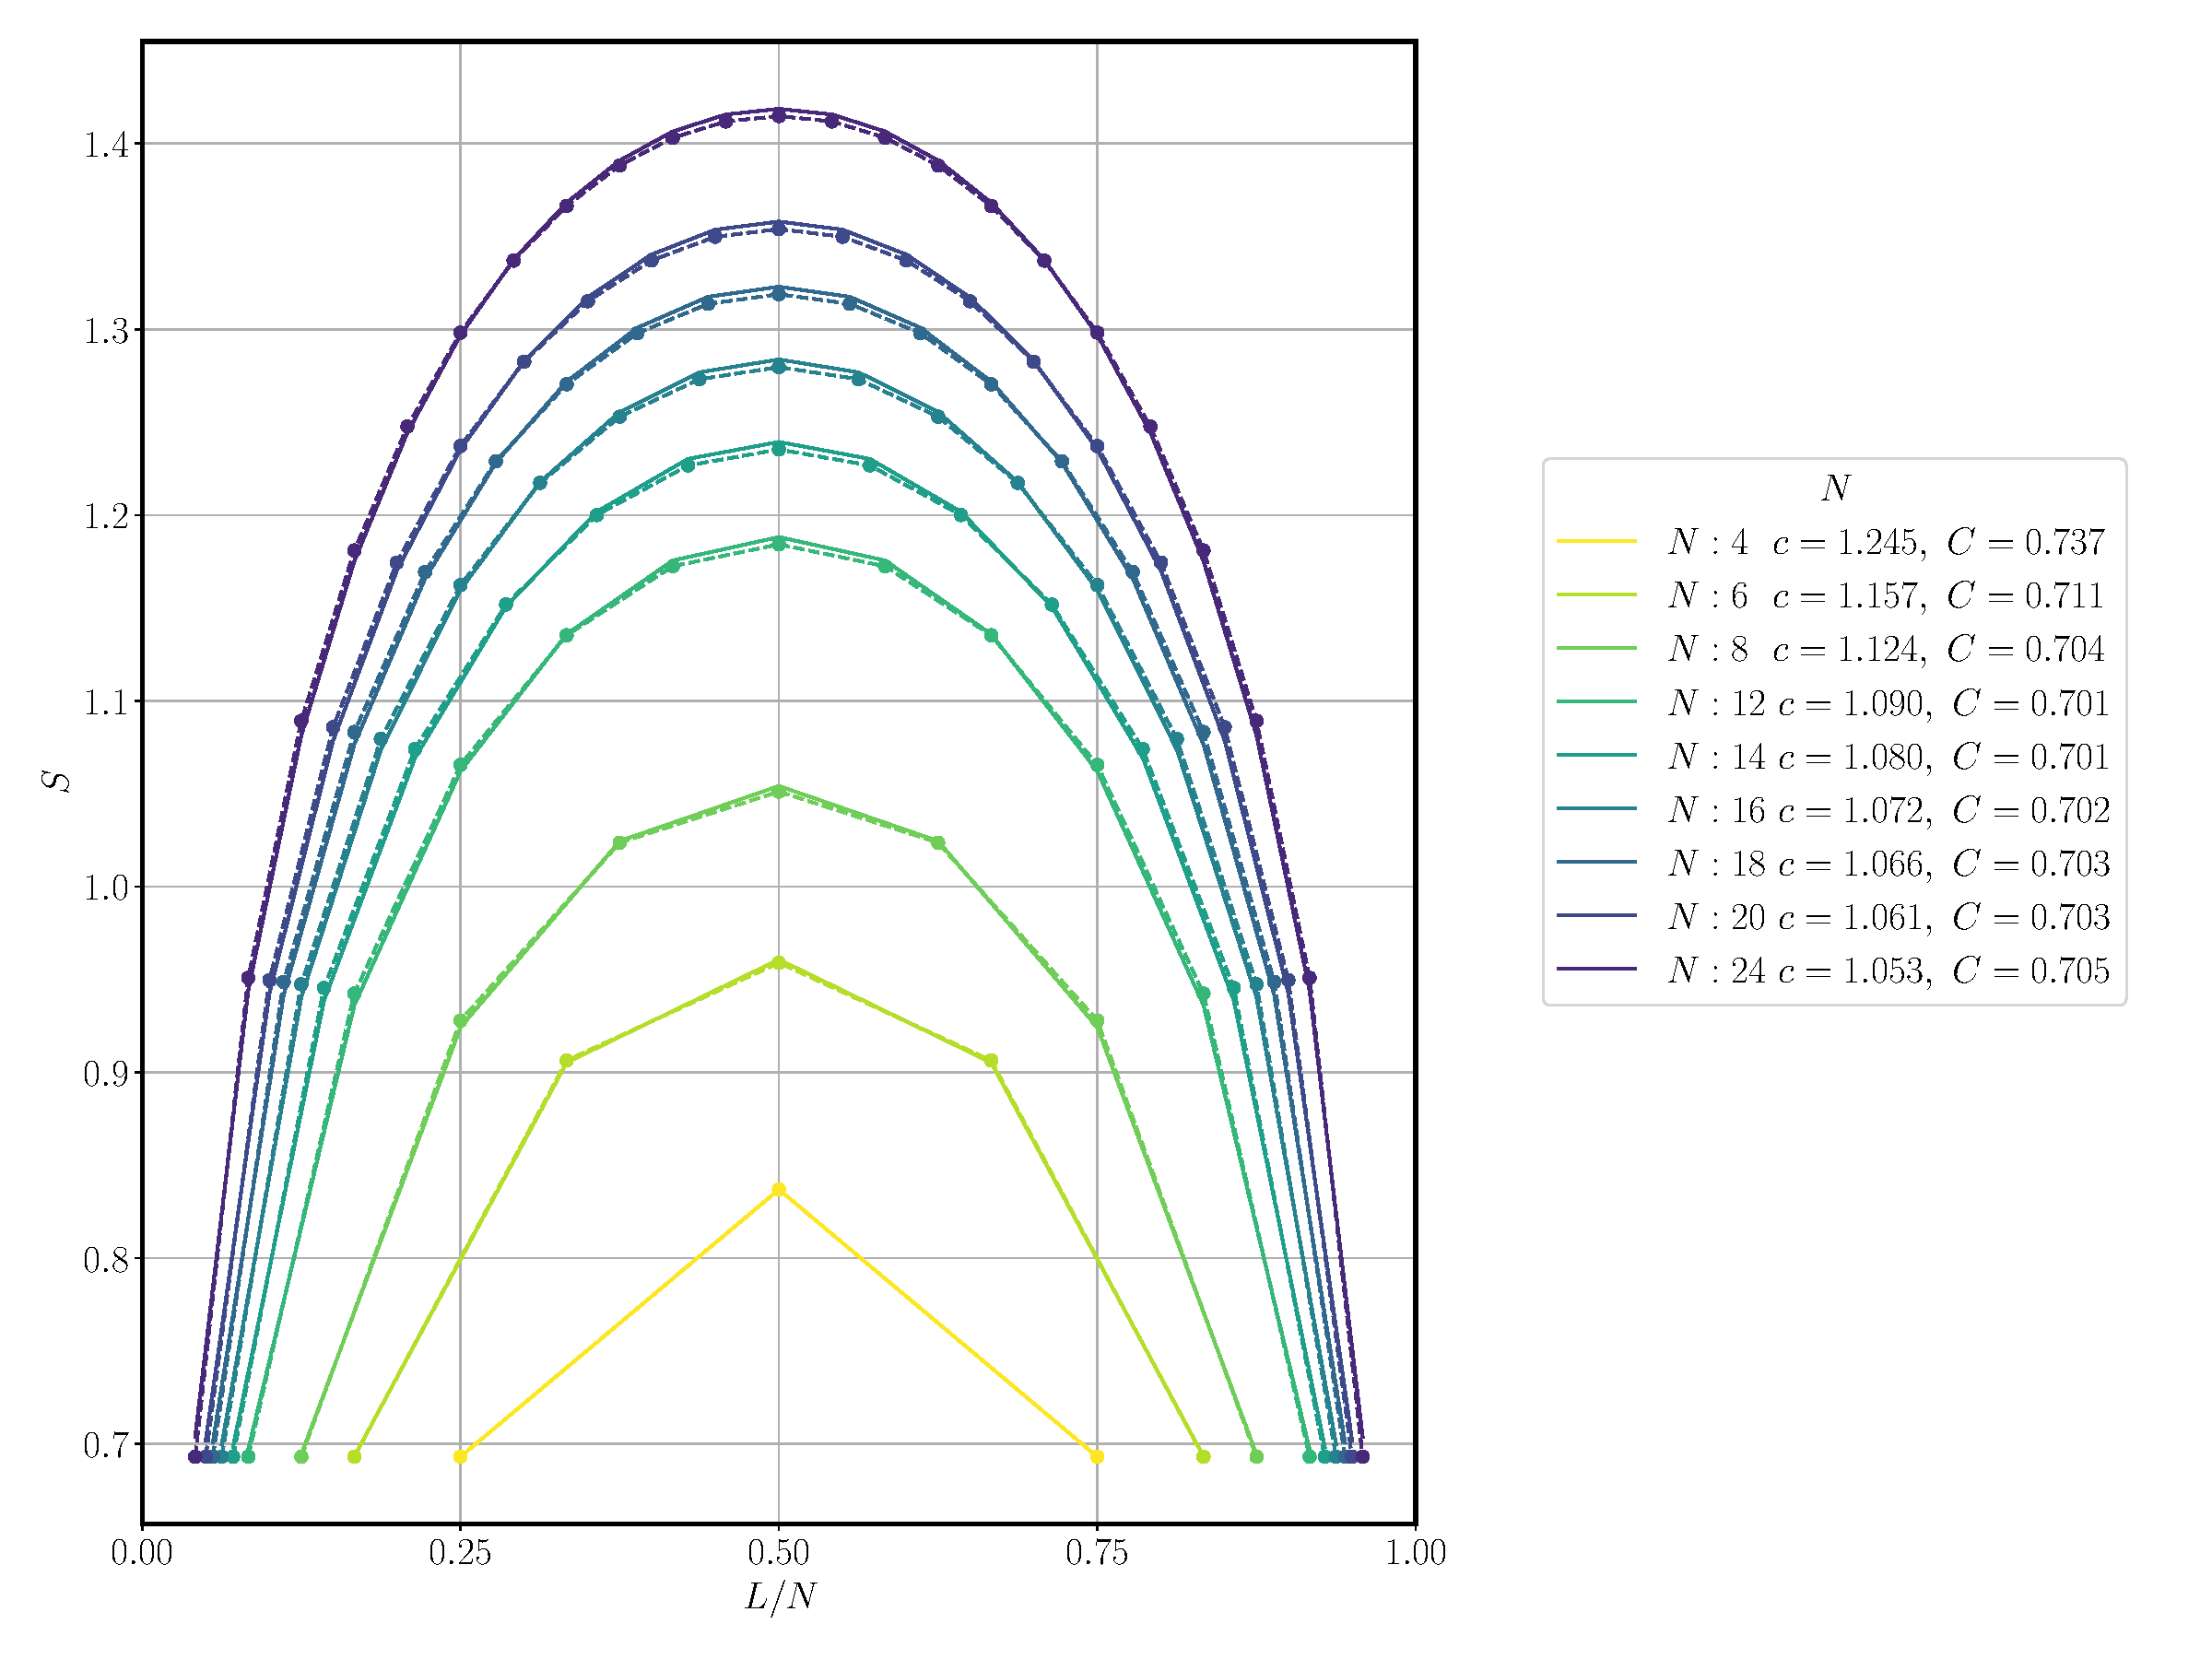
\includegraphics[width=1\textwidth]{figures/ah/entanglement__partition__N__U__J.pdf}
  \caption{Entanglement entropy for the AH model as a function of the partition size, for various system sizes. Shown are fitted curves of the entanglement scaling relation, with fitted central charges and corrections.}
  \label{fig:ah_entanglement_partition}
\end{figure}


\subsection{Anisotropic Heisenberg Model Entanglement Scaling}
We now investigate the scaling of the entanglement entropy for the anisotropic Heisenberg model with $\Delta/J_{\perp} = 1/2$. Shown in \cref{fig:other_entanglement_partition} is the entanglement entropy scaling for $4 \leq N \leq 24$. We observe the entanglement behaviour fits almost perfectly with the scaling in \cref{eq:entropy_scaling}, and the central charge approaches the known value \cite{Cole2017} of $\boxed{c_{\textrm{XXZ - Para}} = 1}$ as the system size increases, and particularly converges for $N>14$. This model has parameters within the paramagnetic phase of the XXZ model, and its central charge estimate confirms it is within this universality class, and is exhibiting some kind of critical behaviour if its entanglement is scaling as if it is conformal. It is also interesting to observe that the corrections $C$ appear to be independent of system size, indicating that if there are any corrections, they may only depend on dimensionless ratios $L/N$.
\begin{figure}[H]
  \centering
  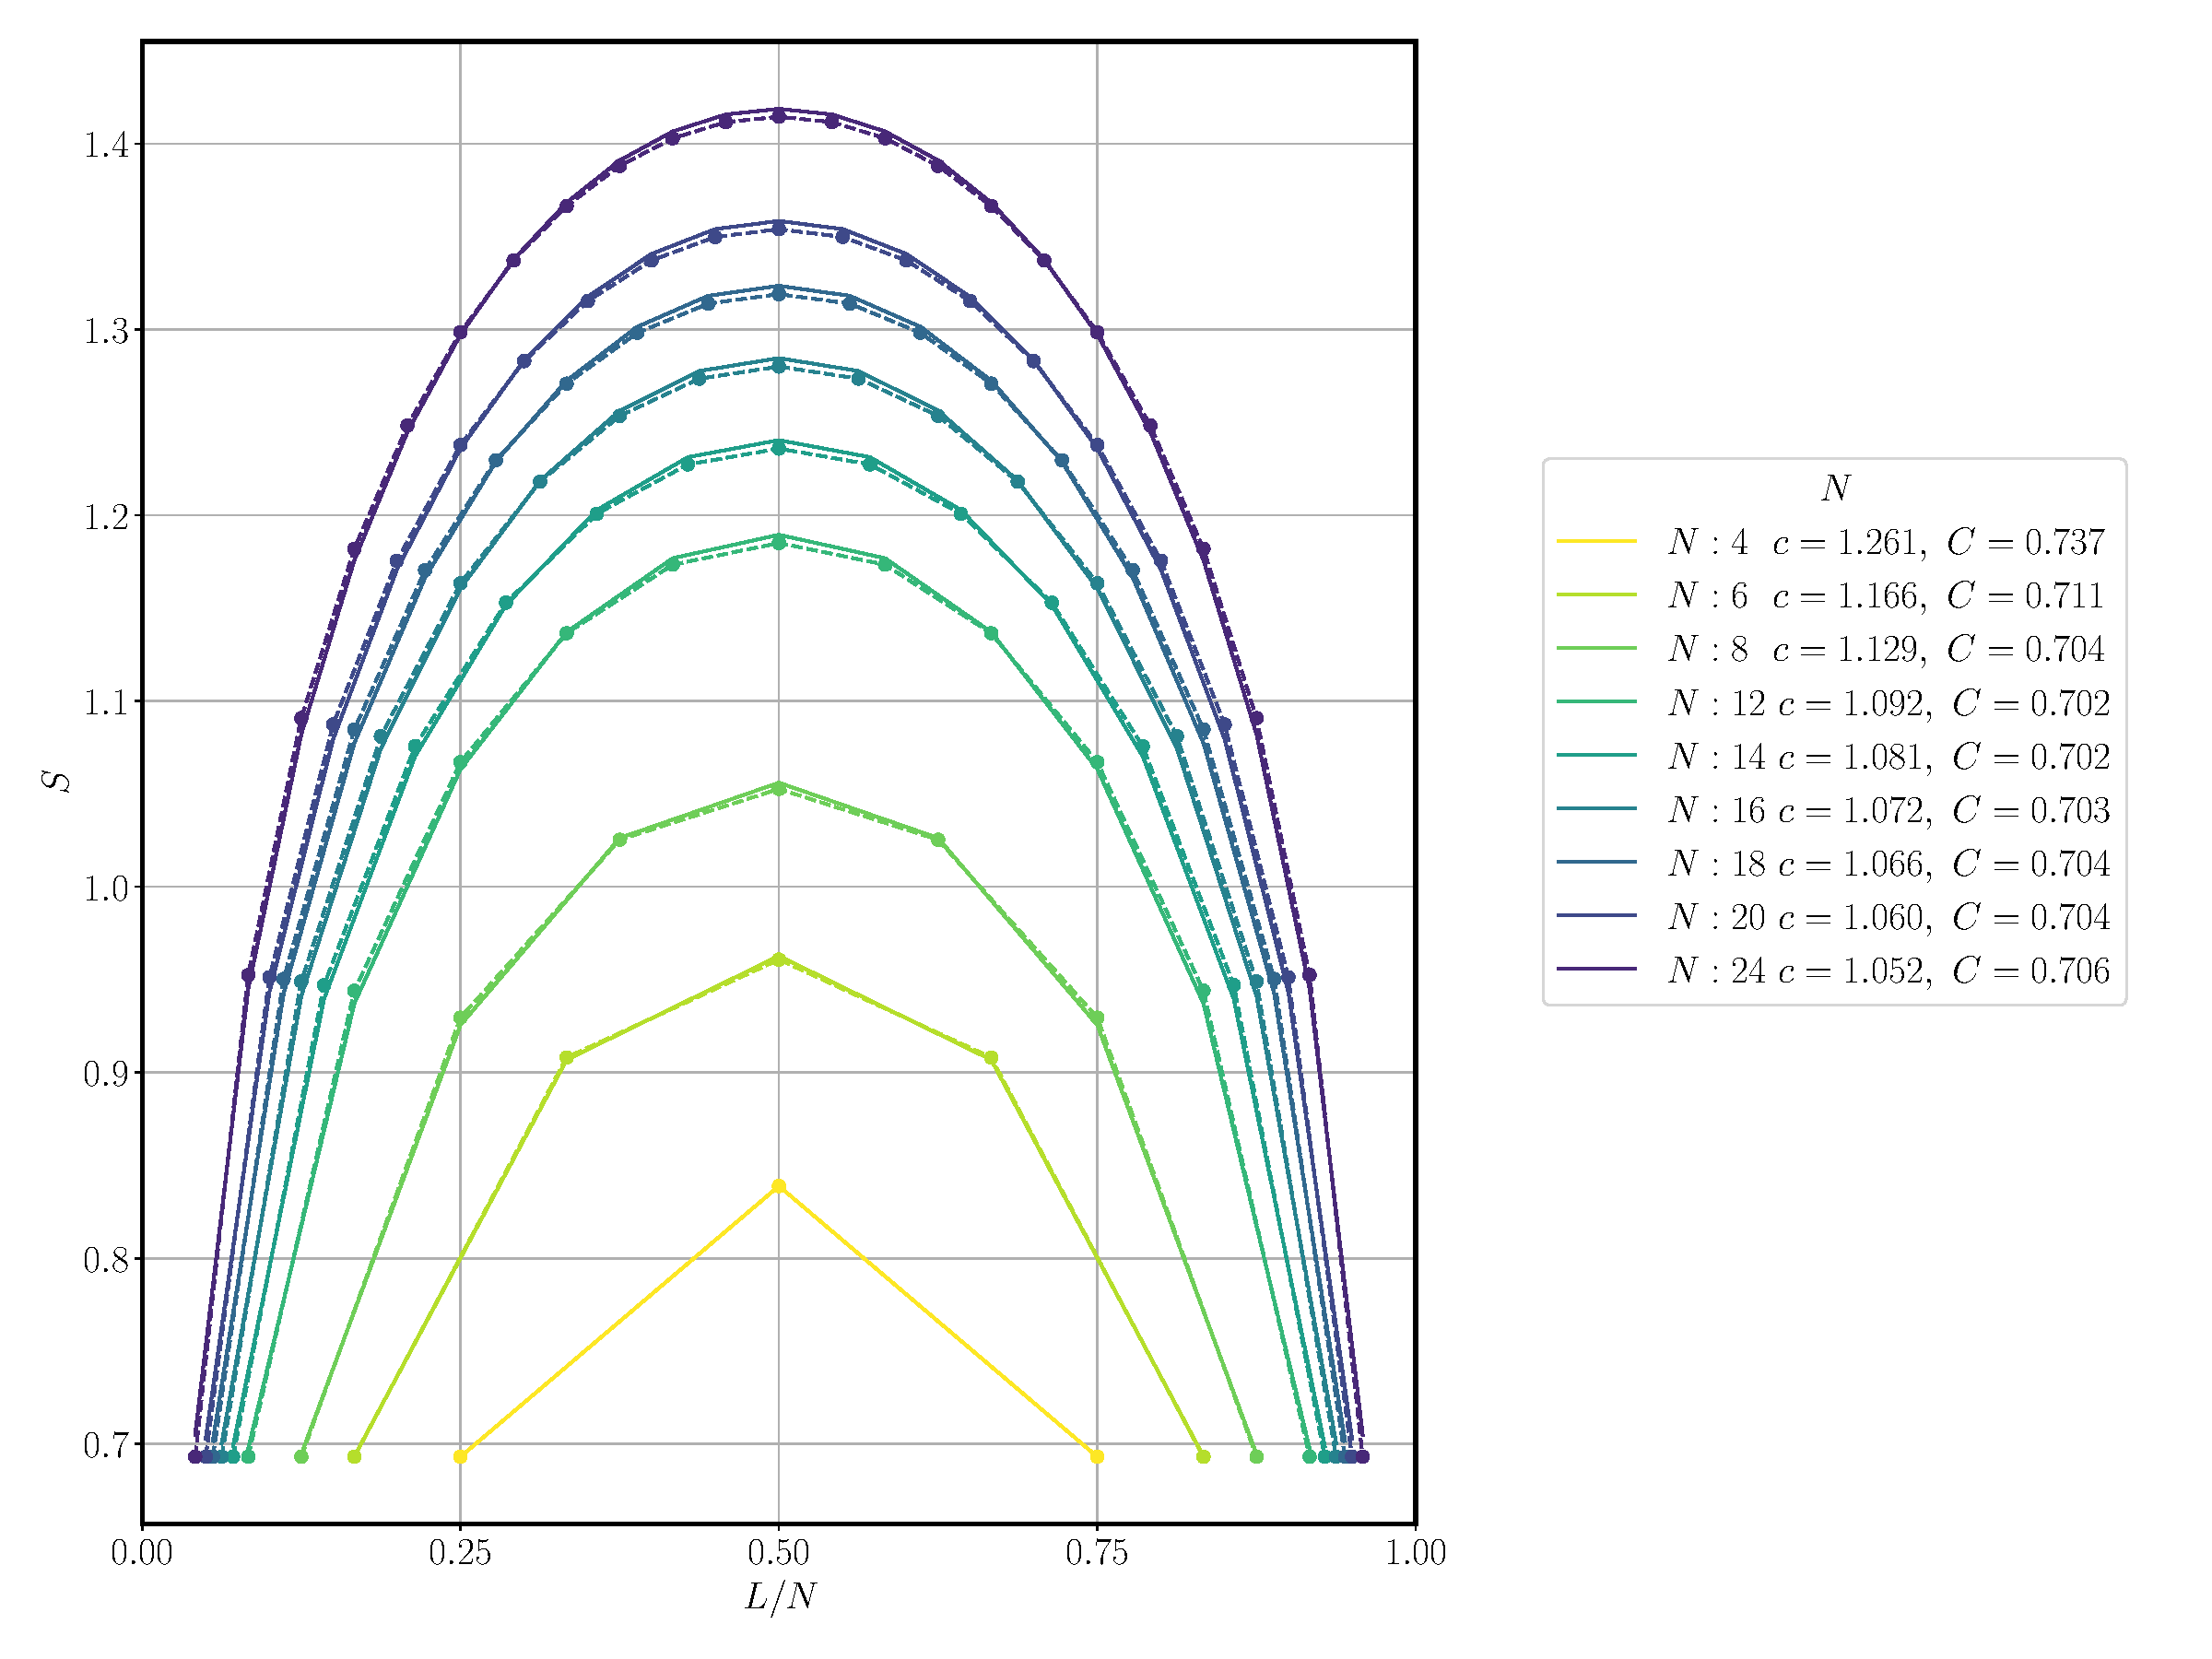
\includegraphics[width=1\textwidth]{figures/other/entanglement__partition__N__U__J.pdf}
  \caption{Entanglement entropy for the anisotropic Heisenberg model with $\Delta/J_{\perp} = 1/2$, as a function of the partition size, for various system sizes. Shown are fitted curves of the entanglement scaling relation, with fitted central charges and corrections.}
  \label{fig:other_entanglement_partition}
\end{figure}
Therefore, the studies of the entanglement entropy with bipartition size and system size confirm the theoretical central charge predictions for the Ising model, and anisotropic Heisenberg models within the paramagnetic phase. Further investigations of a finite size scaling analysis of how the central charges and corrections depend on $C$ and $L$ would be interesting to understand the full entanglement scalings.




\newpage
\section{Many Body Localization}
We now investigate the ferromagnetic Heisenberg model with $\Delta/J_{\perp} = 1$, with local random longitudinal fields $h$
\begin{align}
  H_{\textrm{H}} =&~ -J\sum_{<ij>} S_{i} \cdot S_{j} - \sum_{i} h_{i}S^{z}_{i}, \label{eq:heisenberg_hamiltonian}
\end{align}
where we choose the random local fields to be uniformly distributed, with magnitude $\abs{h/J} \leq W/J$.

We aim to learn the entanglement entropy scalings with system size for different random field magnitudes $W/J$, in both the ground states and excited states at the interior of the energy spectrum. We perform $R = 100$ realizations of each configuration and to ensure interpretable comparisons between realizations, we choose the energy eigenstate $\epsilon$ as a proportion of the total spectrum for that realization. This involves first finding the extremal minimum and maximum eigenvalues, and for a fixed proportion, finding the realization's eigenvalue that is close to some proportion of that range. 

This search for the interior eigenvalues $0 \ll \epsilon \ll 1$ is computationally expensive because, as discussed in the Numerical Methods section, it involves an inversion of the Hamiltonian matrix. However, this model retains an $U_z(1)$ symmetry and conserves $S^{z}$. Therefore, although we will be analysing both ground state and excited states, we will assume we will remain within a sector of constant $S^z$, and choose the $S^{z} = 0$ subspace. This aligns with the approaches from similar studies by Luitz \emph{et al.}\cite{Luitz2014}. 

Due to these constraints of many realizations required and computational expensive eigenvalue searches, for $W/J = 1/2,3,9$, and eigenstates at proportions $\epsilon = 0,0.2,0.5,0.7$, only system sizes of $6 \leq N \leq 16$ for all configurations could be simulated within the time constraints. For $W/J = 1/2$ and $\epsilon = 0, 0.2, 0.5$, $N = 18$ was simulated, however future work should complete the study, with significantly more realizations to observe the true entanglement behaviour. A rough estimate with $4 \leq N \leq 12$ for $R = 1000$ realizations was also computed (and the efficient implementation allowed this study of $O(5 \cdot 10^4)$ realizations to completed in under $2$ minutes), however similar results with high variance were obtained.

\subsection{Eigenstate Thermalization Hypothesis and Many Body Thermalization}
For this study, we aim to understand the distinction between states obeying the eigenstate thermalization hypothesis (ETH), and obeying the more exotic Many Body Localization (MBL). MBL\cite{Abanin2018} states have many fundamental different properties from typical spin systems which have been studied. Unlike spin systems which typically have observables and correlation functions that vary smoothly with the energy eigenstates from one state to an adjacent state, MBL states can have can have observables that fluctuate greatly between adjacent states \cite{Abanin2018}. A key feature of thermalized states is that they also approach being ergodic, and almost the entire state space is accessible, and excited states tend to be highly entangled, leading to the behaviour of entanglement scaling with the volume of the system. In contrast, MBL states tend to remain localized, and perturbations are shown to only propagate locally and decay exponentially from the source, leading to product MBL states that are perturbed remaining roughly product states, with their entanglement not increasing as it would in ETH states.

To analyse conventional states, methods such as mappings to spinless fermions or bosons, such as the Jordan Wigner transformations, are performed. These methods are appropriate due to being exact for many spin-models, and do not have constraints on any locality, however can lead to many difficult, non-local equations to solve to determine the spectrum.

MBL states, being much more local and having less entanglement, mean they can be mapped to product states through unitary transformations, leading to roughly local integrals of motion since the same roughly local unitary transformations can be used to diagonalize the Hamiltonian \cite{Abanin2018}. The unitary transformations required to diagonalize conventional ETH states are highly non-local, in order to depict the large volume-law entanglement present in these states. These local integrals of motion can be shown to be exact, in particular for all energy scales, and unlike conventional methods that are typically only accurate perturbatively in large or small coupling regimes, these MBL methods are much more universal, and is much more robust to perturbations.

Therefore, it is important to study MBL states, and to confirm their area law entanglement scalings, as that will allow the local integral of motion approach to be used and for more interesting localized properties to be discovered.

\subsection{Random Field Heisenberg Model Area and Volume Law Entanglement Scaling}
Shown in \cref{fig:heisenberg_entanglement_N} are the resulting entanglement entropy per site scalings with system size for the various random field magnitudes and energy spectrum proportions, at bipartition sizes of $L = N/2$. In order to determine whether the entanglement for a given eigenstate scales with the area or the volume of the bipartition size, the entanglements are normalized by the system size $N$, and therefore $\boxed{\textrm{area laws will show decreasing } S/N \textrm{ vs. } N}$, and $\boxed{\textrm{volume laws will show constant } S/N \textrm{ vs. } N}$. It is hypothesized that for $W/J > \tilde{W}/J \approx 3$, there will be a phase transition from excited states exhibiting volume law entanglement, to exhibiting area law entanglement scaling \cite{Abanin2018}.

There are severe effects from not simulating adequate realizations, however there are clear trends of area and volume laws for various configurations based on the general increases of the entanglement curves with system size.. For $W/J = 0.5 < \tilde{W}/J$, both the ground state obey the expected area laws, and excited states are shown to obey the expected volume laws. These realizations have the least variance, and show the clearest trend of remaining roughly constant, or slightly increasing with system size. For $W/J = 3 \approx \tilde{W}/J$, the ground state and first excited states also obey the expected area laws, and then the excited states also obey the expected volume laws. The exact critical point could be determined from a more sophisticated finite-size scaling, with many finely spaced $W/J$ values to determine the exact point at which the volume laws for excited states are no longer followed.

For $W/J = 9 > \tilde{W}/J$, there is some evidence of the excited states exhibiting the novel area laws, particularly for higher energies $\epsilon = 0.7$. However, the error bars on all plots are very large, and significantly more realizations would be required to confirm this conjecture,and to observe clear, monotonically decreasing curves indicating a definite area law.
\begin{figure}[H]
  \centering
  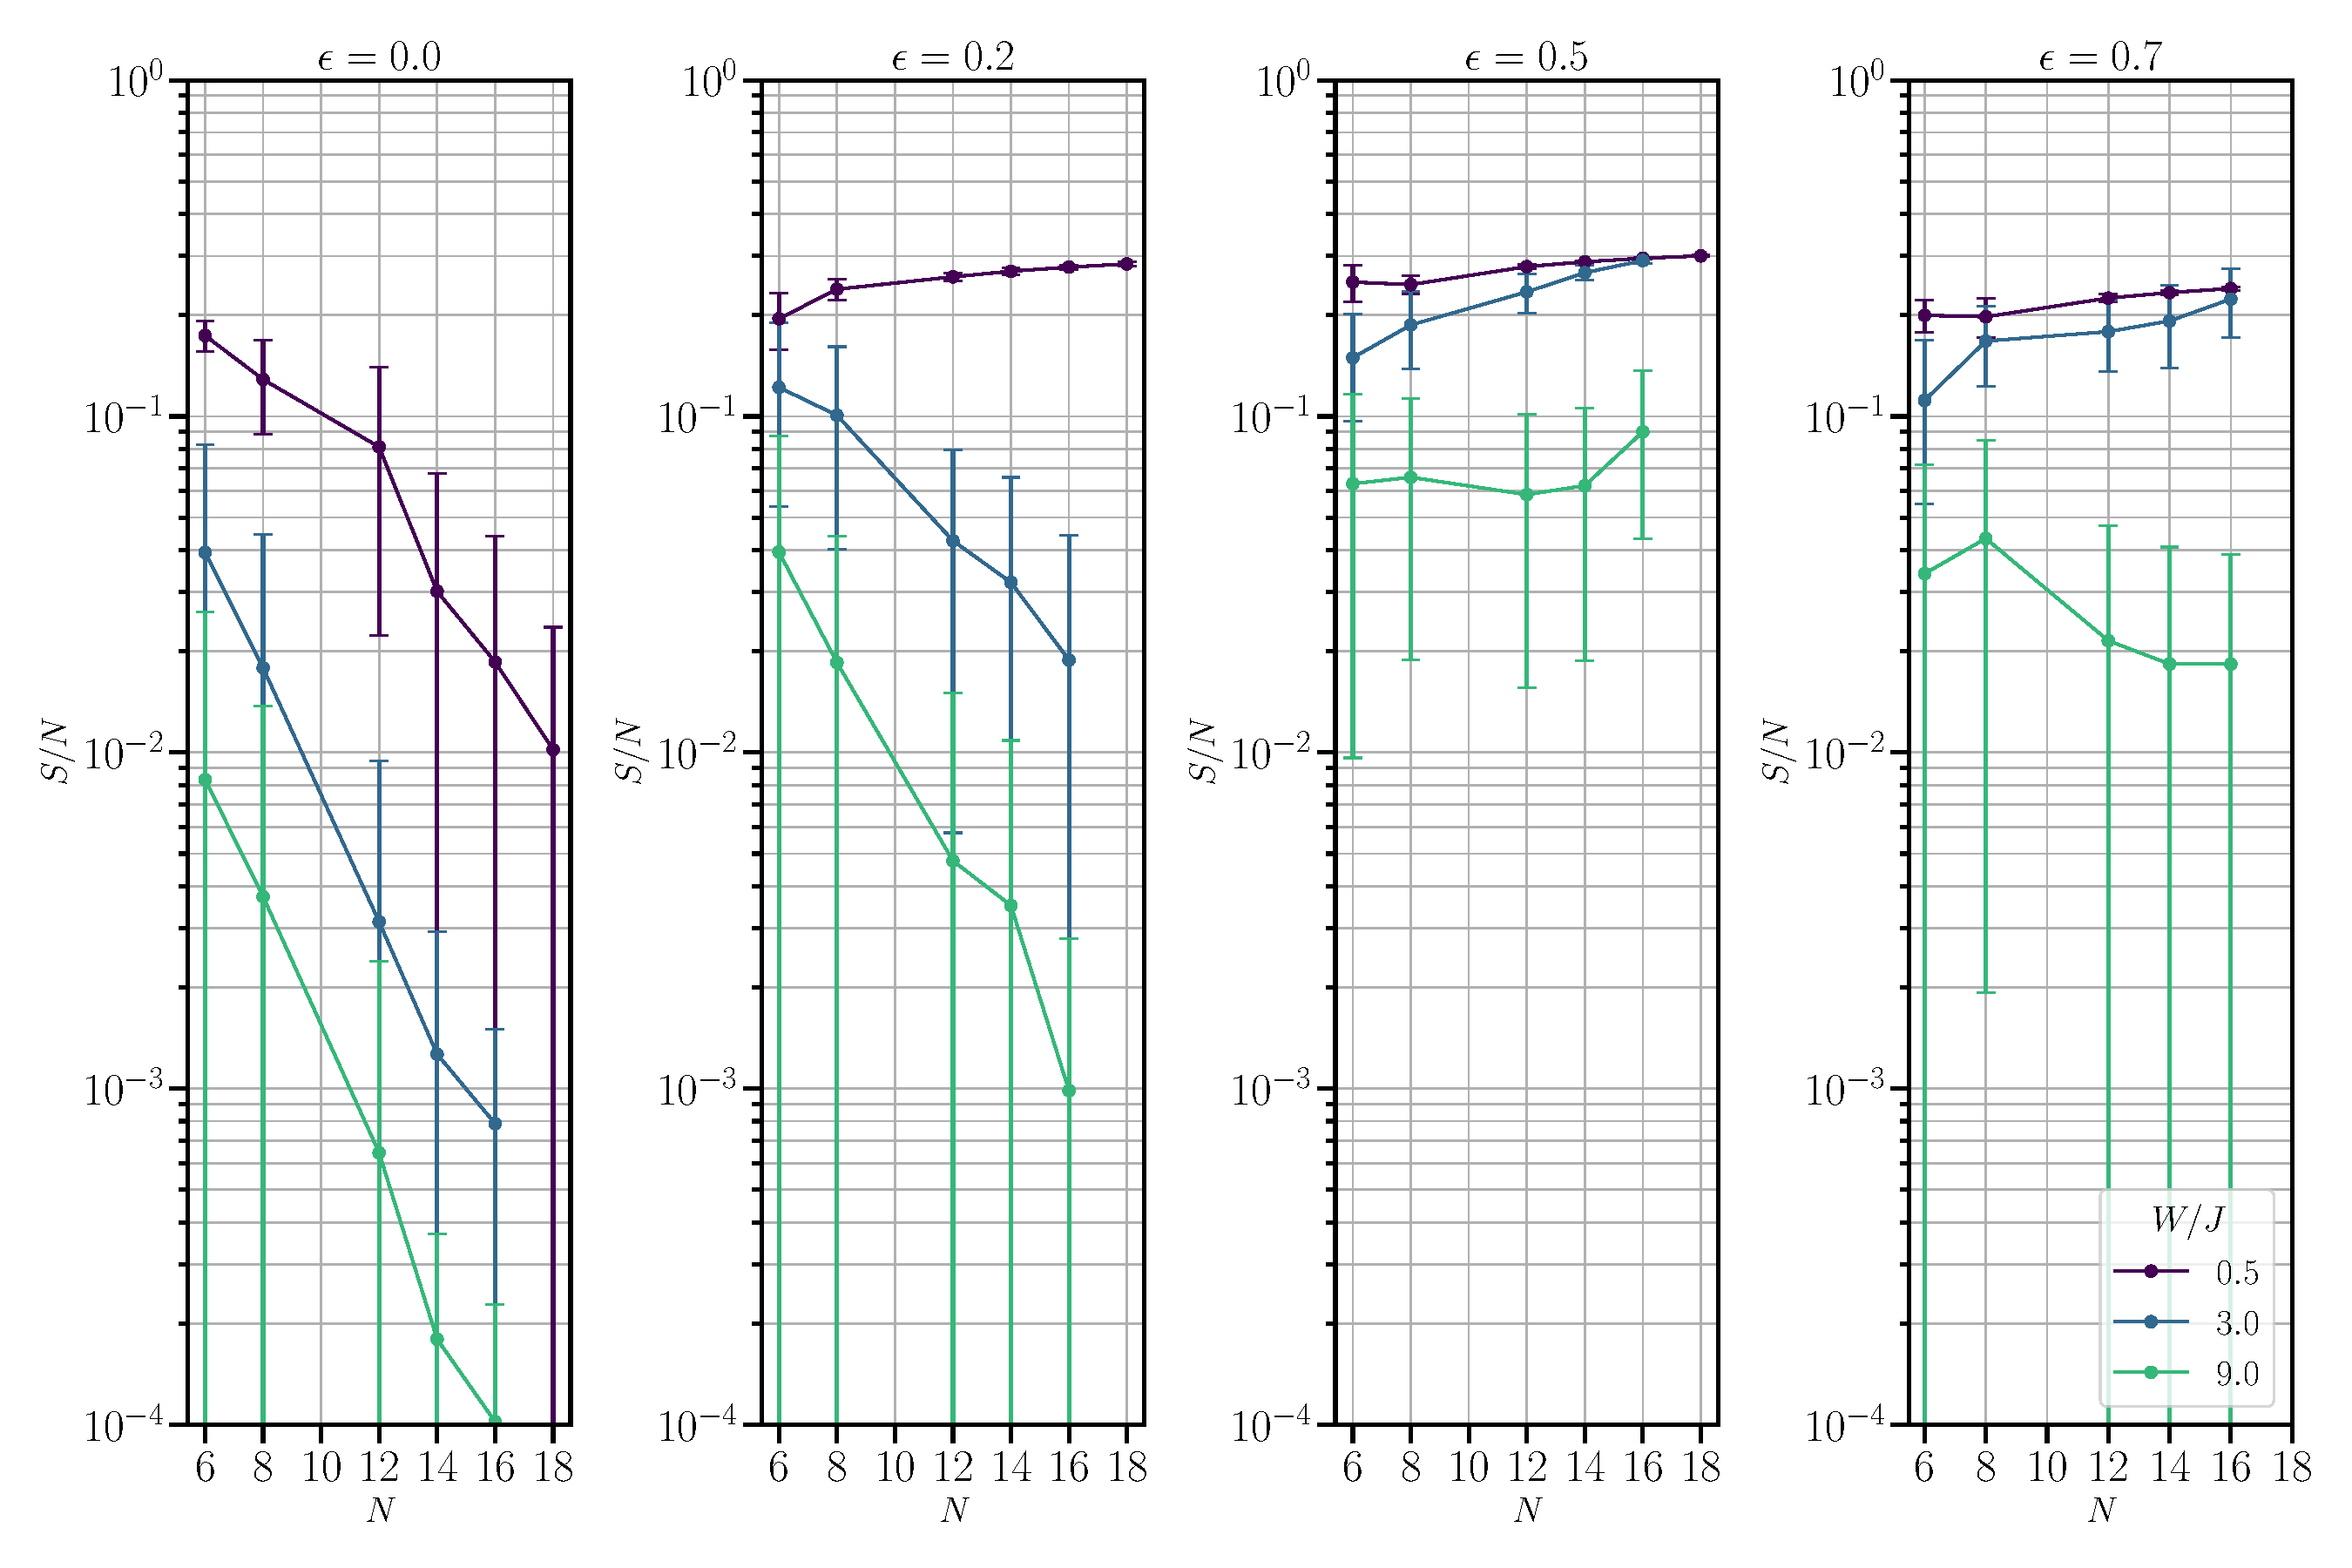
\includegraphics[width=1\textwidth]{figures/heisenberg/entanglement__N__U__J__h__sigma.pdf}
  \caption{Entanglement entropy per site for the ferromagnetic Heisenberg model with random longitudinal fields of maximum magnitude $W/J$, as a function of system size. Shown are different eigenstates at different regions of the spectrum range of each of the $R = 100$ realizations.}
  \label{fig:heisenberg_entanglement_N}
\end{figure}


\newpage
\section*{Numerical methods} \label{sec:numericalmethods}
\addcontentsline{toc}{section}{Numerical Methods}

A diagonalization library is implemented in the \emph{C++} language, which uses the \emph{eigen} \cite{eigen} library for base matrix data structures and eigen-solver wrappers. Please refer to \href{https://github.com/mduschenes/diagonalization}{github.com/mduschenes/diagonalization} for the library repository. The diagonalization is performed for sparse real matrices using the \emph{Arpack} Fortran library \cite{Lehoucq1998}, and the backend for linear-algebra operations, is the state of the art \emph{Intel-MKL} version of the \emph{BLAS} and \emph{LAPACK} libraries, as well as the \emph{openMP} library for multi-core parallelization. Other external libraries used include \emph{cppitertools} for iterating over all simulation configurations, \emph{hdf5cpp} for saving all simulations in a single compressed \emph{hdf5} format, and several optimization features in \emph{c++17} which require the GNU compiler \emph{g++} version $\geq 9.5$.

The computationally intensive operations of the matrix assembly, diagonalization, observable computation, and iterations over different simulations configurations is performed within \emph{c++}, and then saved simulation outputs in an \emph{hdf5} file are passed to a \emph{python} script which post-processes the simulations, including sorting and averaging over simulation realizations, performing fits of the data, and plotting results. 

The computationally intensive operations consist of initializing a \emph{Hamiltonian} class. First the state space and model parameters and lattice can be setup using the \emph{setup()} function. The Hamiltonian matrix can then be assembled using a parallelized sparse matrix initialization scheme and efficient bitwise operations \cite{Sandvik2010,Jung2020} with the \emph{set()} function. The explicit diagonalization for $k$ eigenvalues at a desired point in the spectrum is conducted with the \emph{eig()} function. Observables with the eigenstates are then computed with the \emph{compute()} function. Finally, all observables and model parameters are saved to a group in an \emph{hdf5} file using the \emph{dump()} function.

The workflow can be performed with a single \emph{make process} command, which runs the TFIM model for various transverse fields and system sizes, and saves each simulation, and runs the post-processing, and produces each of the TFIM figures shown in this work. The commands \emph{make run} or \emph{make plot} performs solely the computations or post-processing respectively. 

Alternatively, a custom Hamiltonian class \emph{<model>} in the \emph{src/hamiltonian.hpp} and \\\emph{src/hamiltonian.cpp} files can be implemented with \emph{setup, set, compute} class functions, as well as a main file \emph{src/<model>.cpp} can be implemented. Adding \emph{<model>} to the \emph{PROGAM} variable of the makefile, allows for this model to be run with the commands \emph{make <model>}, \emph{make run\_<model>}, or \emph{make plot\_<model>}. This modularity allows for new Hamiltonians to be studied very efficiently within one uniform workflow, with only small additions necessary for custom models.

The workflow is highly efficient, and on an $8$-core \emph{i7 Intel} processor with $32$ Gb of memory, for up to $N=16$ sizes, each simulation, consisting of initialization, assembly, diagonalization, and all observable calculations takes less than $0.5$ seconds for finding extremal eigenvalues, and the sparse data structures ensures only about $3\% \approx 30$ Mb of memory are used. For $16 < N < 20$ sizes, each simulation takes less than $10$ seconds, and when the matrices are block-diagonal, total sizes of $N \leq 24$ can be reached with similar run-times, and only after $ N>24$ sizes are $90\% \approx 30$ Gb of memory are used. When finding eigenvalues in the interior of the spectrum, the \emph{shift-invert} Lanczos method is implemented, which involves slow matrix inversions, and makes each iteration take up to several minutes for $N>16$, making large simulation sweeps infeasible. For example, the sweeps of transverse fields for the TFIM up to $N=16$ sizes take a few seconds, for up to $N=20$ sizes take less than an hour, and the final entanglement area and volume law scalings, which involve $O(10^4)$ simulations, the simulations had to be run for several days, and was not able to be completed for all simulation realizations.

Future progress on the library includes implementing the \emph{Arpack} Lanczos eigensolver for complex, sparse matrices. Currently, the \emph{eigen} library only includes a wrapper for the real version of the hermitian and sparse Arpack eigensolver, and for more complicated Hamiltonians, this is essential for viability of the library. Fortunately, many finite dimensional (in particular spin based) models can be described by strictly real, symmetric Hamiltonians. Furthermore, fortunately due to the Perron-Frobenius theorem, for these real, symmetric Hamiltonians, the ground eigenstates have strictly real coefficients, and this allows for a slight speed up for observable computations. A general lattice class would also be useful to implement efficient assembly of Hamiltonians on $d$-dimensional lattices. The entanglement calculations are also only currently for $d=1$ dimensional systems, and take advantage of the simplified partial trace and SVD computations that can be performed on a bi-partitioned pure state, and efficient extensions to higher dimensions should be implemented. A more parallelized and efficient matrix inversion procedure should also be implemented for efficient eigenvalues in the interior of the spectrum.


\newpage
\section*{Conclusions} \label{sec:conclusions}
\addcontentsline{toc}{section}{Conclusions}
This work studied various finite dimensional spin $1/2$ system on a finite size lattice. Various ground state properties of the transverse field Ising (TFIM) model were analysed, including the scaling of the gap at criticality to its first excited state for finite size systems of $\tilde{\Delta} \sim N^{-1}$, and the presence of a critical point at a transverse field of $\tilde{h}/J = 1$. The TFIM entanglement scaling as a function of bipartition sizes $L/N$ in the system were also observed to almost exactly follow the conformal scaling law at criticality, with a confirmed central charge of $c_{\textrm{TFIM}} = 1/2$. 

Anisotropic Heisenberg (XXZ) models, including the XY model and antiferromagnetic isotropic Heisenberg (AH) model were also studied, with their ground state energies shown to quadratically approach their thermodynamic values with finite system size as $\Omega \sim N^{-2}$. The XY and AH, as well as other models within the parametric phase of the full anisotropic Heisenberg models with longitudinal and transverse coupling ratios $\Delta/J_{\perp}$, were also shown to be within the same universality class, to have entanglement the scales conformally with the bipartition size, and have a confirmed central charge of $c_{\textrm{XXZ - para}} = 1$.

Finally, the transition between eigenstate thermalization and many-body localized phases for random-field Heisenberg models with increasing random field magnitudes are studied in terms of entanglement scaling laws. The approximate area law for thermalized ground states and volume law for the thermalized excited states is shown, in contract to the approximate area law for the many-body localized excited states for greater disorder $W/J > \tilde{W}/J \approx 3$. An increased number of realizations of each configuration are necessary to truly confirm these results.

Ultimately, performing analyses of many-body systems with numerical methods has many advantages and disadvantages compared to analytical methods. Utilizing numerical methods has the disadvantages of performing certain computations such as integrals and determining eigenvalues within the interior of the spectrum, can be occasionally easily performed analytically, but are very computationally expensive to estimate numerically. There are also several floating point error issues that arise, particularly when distinguishing degenerate subspaces of the system, and determining whether systems have a gap, or are in fact degenerate. Finally, the efficiency of performing computations in general, including the implementation can be a very inefficient process, if analytical reasoning and scaling arguments can achieve similar results with similar levels of confidence.

However, this study shows that numerical methods have more advantage than disadvantages. First, personally implementing the diagonalization and computation algorithms and ensuring they are memory and time efficient really allows us to understand how difficult quantum systems are to study, and to really see the subtleties in interpreting their results. For example, the subtleties with the ground state degeneracies in finite size systems really show the effects of perturbation theory. Furthermore, performing finite size-scaling analysis and performing regression for coefficients allows us to understand critical exponents and how quantities are related to each other in a way that can be opaque when making ansatz about scaling in analytical studies. Finally, numerical studies allows us to perform experiments and to test whether certain conjectures may be valid, and estimate quantities that have no closed form. This is especially enlightening in the case of estimating ground state energies, where even if we did not have a closed form as we did in the models studied, the convergence with system size would allow us to estimate energies of other similar models. Numerical methods have been shown to be an essential tool for physicists to further their understanding of many-body systems.



%%%%%%%%%%%%%%%%%%%%%%%%%%%%%%%%%%%%%%%%%%%%%%%%
% \newpage
\pagestyle{bibliography}
\bibliography{main}

%%%%%%%%%%%%%%%%%%%%%%%%%%%%%%%%%%%%%%%%%%%%%%%%


\end{document}                        